\documentclass{article}

\usepackage{amsmath, amsthm, amssymb, amsfonts}
\usepackage{thmtools}
\usepackage{graphicx}
\usepackage{setspace}
\usepackage{geometry}
\usepackage{float}
\usepackage{hyperref}
\usepackage[utf8]{inputenc}
\usepackage[english]{babel}
\usepackage{framed}
\usepackage[dvipsnames]{xcolor}
\usepackage{tcolorbox}

\definecolor{bubblegum}{rgb}{0.99, 0.76, 0.8}

\colorlet{LightGray}{White!90!Periwinkle}
\colorlet{LightOrange}{bubblegum!20}
\colorlet{LightGreen}{Green!15}
\colorlet{LightBlue}{Blue!15}
\colorlet{LightYellow}{Yellow!15}
\colorlet{LightRed}{Red!15}



\newcommand{\HRule}[1]{\rule{\linewidth}{#1}}

\declaretheoremstyle[name=Theorem,]{thmsty}
\declaretheorem[style=thmsty,numberwithin=section]{theorem}
\tcolorboxenvironment{theorem}{colback=LightGray}

\declaretheoremstyle[name=Proof,]{prosty}
\declaretheorem[style=prosty,numberlike=theorem]{Proof}
\tcolorboxenvironment{Proof}{colback=LightOrange}

\declaretheoremstyle[name=Example,]{prcpsty}
\declaretheorem[style=prcpsty,numberlike=theorem]{Example}
\tcolorboxenvironment{Example}{colback=LightGreen}

\declaretheoremstyle[name=Def]{prcpsty}
\declaretheorem[style=prcpsty,numberlike=theorem]{Def}
\tcolorboxenvironment{Def}{colback=LightYellow}


\declaretheoremstyle[name=Problem,]{prcpsty}
\declaretheorem[style=prcpsty,numberlike=theorem]{Problem}
\tcolorboxenvironment{Problem}{colback=LightBlue}

\declaretheoremstyle[name=Solution,]{prcpsty}
\declaretheorem[style=prcpsty,numberlike=theorem]{Solution}
\tcolorboxenvironment{Solution}{colback=LightRed}

\declaretheoremstyle[
    headfont=\bfseries\sffamily\color{NavyBlue!70!black}, bodyfont=\normalfont,
    mdframed={
        linewidth=2pt,
        rightline=false, topline=false, bottomline=false,
        linecolor=NavyBlue
    }
]{thmblueline}
\declaretheorem[style=thmblueline, numbered=no, name=Note]{note}

\setstretch{1.2}
\geometry{
    textheight=9in,
    textwidth=5.5in,
    top=1in,
    headheight=12pt,
    headsep=25pt,
    footskip=30pt
}
\newcommand\N{\ensuremath{\mathbb{N}}}
\newcommand\R{\ensuremath{\mathbb{R}}}
\newcommand\Z{\ensuremath{\mathbb{Z}}}
\renewcommand\O{\ensuremath{\emptyset}}
\newcommand\Q{\ensuremath{\mathbb{Q}}}
\newcommand\C{\ensuremath{\mathbb{C}}}
% ------------------------------------------------------------------------------

\begin{document}

% ------------------------------------------------------------------------------
% Cover Page and ToC
% ------------------------------------------------------------------------------

\title{ \normalsize \textsc{}
		\\ [2.0cm]
		\HRule{1.5pt} \\
		\LARGE \textbf{\uppercase{Abstract Algebra}
		\HRule{2.0pt} \\ [0.6cm] \LARGE{} \vspace*{10\baselineskip}}
		}
\date{}
\author{\textbf{Author} \\ 
		Persy \\}

\maketitle
\newpage

\tableofcontents
\newpage

% ------------------------------------------------------------------------------
\section{Groups}
% Unfinished, going to include Quiz and Homework questions, midterm questions, and some notes maybe
%
\section{Section 13,14,15}
\begin{Def}
    A subgroup N of G is called a normal subgroup, if a left coset of N is the same as the corresponding right coset of N.
    \\i.e. gN = Ng for all g $\in G$
    \\ We write $N \lhd G$.
\end{Def}

\begin{theorem}
    For any group homomorphism $\phi: G \rightarrow G'$: ker$\phi \lhd G$
\end{theorem}
\begin{Proof}
    1. ker$\phi <$ G.
    \\2. To show that it is a normal, we show show $g(ker\phi) = (ker\phi)g$
    \\And we do it by $\subseteq$ and $\supset$ and we take any$k \in ker \phi$.
    \\ $\subseteq$ : $gk = (gkg^{-1})g $ Then to show $\phi (gkg^{-1}) = e$. The other side is similar. 
\end{Proof}

\begin{theorem}
    Assume $H<G$ The following statements are equivalent:
    \begin{enumerate}
        \item $H \lhd G$
        \item $g^{-1}Hg = H$ for all $g \in G$
        \item  $g^{-1}Hg \subseteq H$  for all $g \in G$
    \end{enumerate}
\end{theorem}

\begin{Def}
    $H \lhd G$. S = $\{ gH \mid g \in H\}$ Define a binary operation on S s.t. $(g_1H) * (g_2H) = (g_1g_2)H$ 
\end{Def}
\begin{note}
       Need to check it is well defined, that is to show take different representative of g1 and g2 we get the same result, which is to consider $g_1H = g_1' H$, $g_2H = g_2'H$
\end{note}


\begin{theorem}
    The map: $\pi: G \rightarrow S = \{gH \mid g\in G\}$ , S is the quotient group that has H as the identity, is a group homomorphism where $H \lhd G$.
    \\The kernel: ker$\pi = H$
\end{theorem}

\begin{theorem}
    Fundamental theorem of group homomorphism. 
    \\Let $\phi: G \rightarrow G' $be a group homomorphism. Then:
\begin{enumerate}
    \item $\phi(G) < G' $
    \item ker$\phi \lhd G$
    \item The quotient group $G/ker\phi $is isomorphic to $\phi (G)$ via the map:
    \\ $\Bar{\phi}: G/ker\phi  \rightarrow \phi(G)$
    \\ $g ker \phi \mapsto \phi(g)$
\end{enumerate} 
\end{theorem}
   % \begin{figure}
   %     \centering
   %     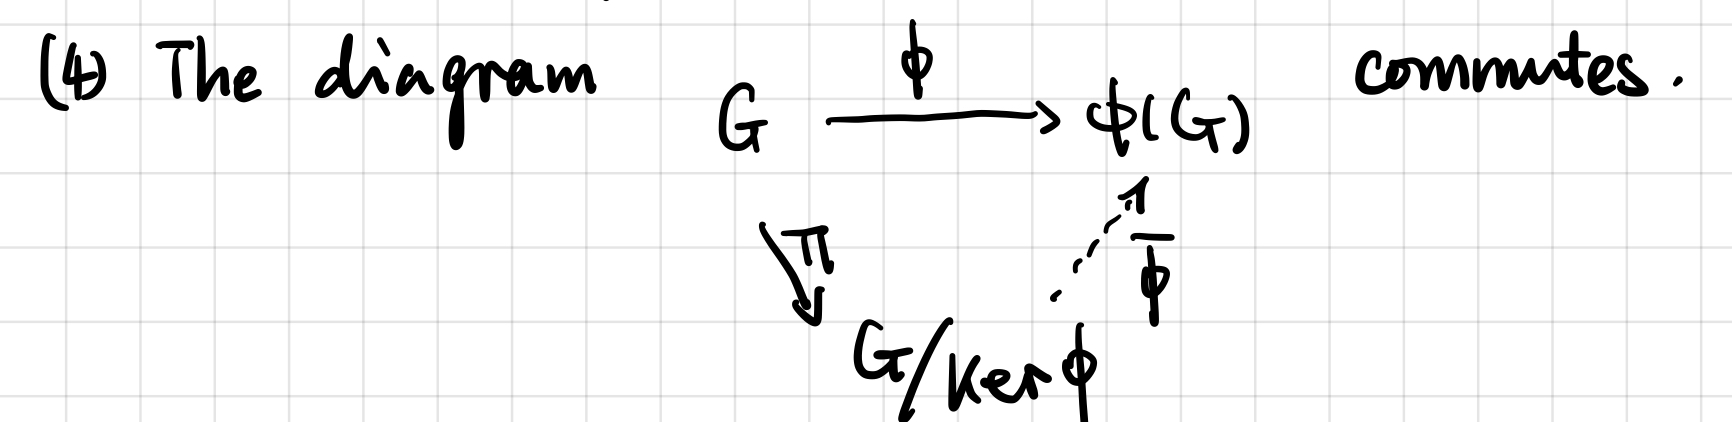
\includegraphics[width=0.5\linewidth]{fig_homomorphism.jpg}
   %     
   %     \label{fig:enter-label}
   % \end{figure}



\begin{Def}
    Automoprhism and adj.
\end{Def}

\begin{Def}
    A group is called simple if it has no proper nontrivial normal subgroup.
\end{Def}
\begin{theorem}
    An, when $n\geq5$ is simple.
\end{theorem}

\begin{Def}
    A maximal normal subgroup of a group G is a normal subgroup M not equal to G s.t. that there is no proper normal subgroup N of G properly contains M.
\end{Def}

\begin{theorem}
    M is a maximal normal subgroup of G $\Leftrightarrow$ $G/M$ is simple
\end{theorem}
\newpage

% ------------------------------------------------------------------------------
\section{Ring}


\subsection{Section 18: Ring & Fields}


\begin{Def}
    A ring $(R, +, \cdot)$ is a set R with two binary operations, addition and multiplication such that the following requirements hold:
    \begin{enumerate}
        \item \\ $(R, +)$ is an abelian group.
        \item \\ $(R, \cdot)$ is associative.
        \item \\ $+ and \cdot $ satisfy left and right distributive law:
        \\ for any $a,b, c \in \R$:
        \\ $a\cdot (b+c) = (a \cdot b) + (a \cdot c)$
        \\ $(a+b) \cdot c = (a \cdot c) + (b \cdot c)$
    \end{enumerate}
\end{Def}

\begin{Example}
    $(0, +, \codt)$ 0 is a trivial ring
\end{Example}

\begin{Example}
    $(\Z / \Q / \R, /\C, + , \cdot)$ are standard ring structures. 
\end{Example}

\begin{Example}
    $(nZ, +, \cdot)$ is a ring and a subring of $\Z$
\end{Example}

\begin{Example}
    $(\Z_n, +, \cdot)$ is a ring.
\end{Example}


\begin{def}
    S is a subring of R if $S\subseteq R$ and closed under + and $\cdot$
\end{def}

\begin{Def}
    A map $\phi: R \rightarrow R'$ for rings R and R' is called a ring homomorphism  if 
    \\1)  $\phi (a+b) = \phi(a) + \phi(b)$
    \\2) $\phi (a \cdot b ) = \phi(a) \cdot \phi(b)$ for all $a, b \in R$
    \\(1) is equivalent to $\phi:(R, +) \rightarrow (R', +') $ is a group homomorphism. ker$\phi$ is the kernel for such group homomorphism. 
\end{Def}

\begin{Example}
    Modulo map $\phi :\Z \rightarrow \Z_n $ is a ring homomorphism. 
\end{Example}

\begin{Proof}
    $\phi$ is a group homomorphism.
    \\ $\phi(ab) ?= \phi(a) \cdot \phi(b)$
    \\ we can denote $a = ln + \phi(a)$, $b = mn + \phi(b)$ as elements in $\Z_n$
    \\ $a \cdot b = (ln + \phi(a)) \cdot mn + \phi(b) = ln(mn + \phi(b)+\phi(a)mn + \phi(a)\cdot \phi(b)) = \phi(a)\cdot \phi(b) $    
\end{Proof}

\newpage
\begin{Def}
    A bijective ring homomorphism is called a ring isomorphism.
\end{Def}
\begin{Example}
    $(\Z, +) \cong (3\Z,+)$ is a group isomorphism but not a ring somorphism. 
\end{Example}

\begin{Def}
    A ring $(R, +, \cdot)$ is called commutative if $(R, \cdot)$ is commutative.
    Unital or a ring with unity of $(R, \cdot)$ has the identity for $(R, \cdot)$
    \\ Rmk: Communtativity and unital property are preserced under ring isomorphism.
\end{Def}
\begin{theorem}
    Denote by 1 the unity of the unital ring R.
    \\Then R is trivial iff 1= 0
\end{theorem}

\begin{Example}
    \begin{itemize}
    \hfill 
        \item $\Z_n$ is commutative.
        \item $\C, \R, \Q, \Z $ are unital.
        \item $\Z_n$ is unital.
        \item $n\Z$ is not unital when $n\geq2$
    \end{itemize}
\end{Example}
\begin{Example}
    Show that $\Z_{mn} \cong \Z_m \times \Z_n$ as rings when m and n are coprime. 
\end{Example}
\begin{Proof}
    The group isomorphisms can be shown by mapping generator to generator. 
    $\phi: 1\mapsto (1,1)$ And we show such it is a ring homomorphism too. 
\end{Proof}

\begin{Def}
    Let R be a unital ring with $1\neq 0$:
    \\ A multiplicative inverse of $a \in R$ is an element $b \in R$ so that $a \cdot b = 1 = b \cdot a$
    
\end{Def}

\begin{Def}
    Let R be a untial ring with $1\neq0$.
    \begin{itemize}
        \item An element $u \in R$ is called a unit, if it has a multiplicative inverse. 
        \\Denot by $R^\times = \{u \in R \mid $ u is a unit\}
        \item If $R^\times = R^*$ then R is a divison ring.
        \item If R is commutative, it is called a field.
    \end{itemize}
\end{Def}

\begin{Example}
    $\Z_n$ is commutative unital ring.
    $\Z_n^\times = $\{$m \in \Z_n \mid gcd(m,n) =1 $\}
\end{Example}

\newpage





% ------------------------------------------------------------------------------
\subsection{Section 19: Integral Domains}

\begin{Def}
    In a ring R, if $a, b\in R^*$ satisfy $a \cdot b = 0$ then a, b are called divisors of zero.
\end{Def}

\begin{theorem}
    $\Z_n = \{ 0,1,\cdots n-1\} , m \in \Z_n$ is a divisor of zero iff $m\neq 0$ and gcd(m,n)$\neq 1$
\end{theorem}

\begin{Proof}
    Denote by d= gcd(m,n).
    
    \\$\Rightarrow$ If m is a divisor of zero, there must be a $k \neq 0$ in $\Z_n$ that $mk = ln$.
    \\ If $gcd(m,n) = 1$, $n \mid k$, then $k = 0$ in $\Z_n$. Contradiction. Thus  $gcd(m,n) \neq 1$
    \\$\Leftarrow$ Note that $\frac{mn}{d} =\frac{m}{d} \cdot n $ in $\Z$
    \\there is $[m] \codt [\frac{n}{d}] = [\frac{m}{d} n] = [0]$ in $\Z_n$.
    \\ If $d\neq 1$, $\frac{n}{d} \neq 0 $ in $\Z_n$. We conclude must have $m = 0$
\end{Proof}


\begin{Def}
    An integral domain is a commutative unital ring with $1\neq 0$ and containing no divisor of zero.
   \\ Cor: For any prime number p, $\Z_p$ is an integral domain. 
\end{Def}


\begin{Example}
    Show$ \Z_p$ is a field when p is a prime number. 
\end{Example}
\begin{Proof}
    We only need to show that every nonzero element in $\Z_p$ is a unit.
    \\Take $a \in \Z_p. a\neq 0$ 
    \\Consider the map $\phi_a : \Z_p \rightarrow \Z_p $
    \\ \hspace*{3.5cm} $x \mapsto ax$ in $\Z_p$
    \\ We claim that $\phi_a $ is a bijection:
    \begin{itemize}
        \item $\phi_a$ is injective: $\phi_a(x) = \phi_a(y)$
        \\Then ax = ay $\Rightarrow$ $a(x-y) = 0$
        \\ Since $\Z_p$ is an integral domain and has no divisor of 0, then $a\neq0$
        \\ Thus $x = y$
    \end{itemize}
    \begin{itemize}
        \item $\phi_a$ is a surjective map since $\Z_p$ order is finite and injectivity implis surjectivity. \\ Then it is a bijective map.
    \end{itemize}
    \\Hence there is some $x\in \Z_p$ that $\phi_a(x) = 1$ which is $ax = 1$ and shows that a is a unit. 
\end{Proof}

\begin{theorem}
    Every finite integral domain is a field.
\end{theorem}

\begin{Example}
    $\Z$ is an example of integral domain, but not a field. Note it has infinite order.
\end{Example}

\begin{theorem}
    Every field is an integral domain.
\end{theorem}

\begin{Proof}
    That is to show for $a, b\in F, ab = 0 $ either $ a=0 $ or $ b = 0$
    \\If $a\neq 0$ then a is a unit, thus $a \cdot a' = 1 = a' \cdot a$.
    \\Then $a'(ab) = a'0 = 0 = 1(b) = b$
\end{Proof}

\begin{Def}
    Let R be a ring. Define the charateristic of R as:
    \\ char(R) = min \{$n \in \Z^+ \mid  n \cdot a = 0$ for all $a\in R$\}
    \\Define char(R) = 0 when such set is empty.
\end{Def}

\begin{Example}
    char($\Z_n$) = n, char($\Z$) = 0
\end{Example}
\begin{theorem}
    For a unital ring R,
    \\char(R) = min \{$n \in \Z^+ \mid  n \cdot 1 = 0$ for 1 is unity $\in R$\}
\end{theorem}

\begin{Proof}
   Easy to check if $\{n \in \Z^+ \mid n\cdot 1 = 0\} = \varnothing$ Then $\{n \in \Z^+ \mid n\cdot a = 0\} =\varnothing$ the char(R) does not exists = 0.
   \\Other wise: denote $m = min \{n \in \Z^+ \mid n\cdot 1 = 0\} $ Want to show that $ma = 0 $ for all $a\in R$.
   \\Since ma = $a+a+...a $(for m times) = $a*1 + a*1 +...a*1$(for m times)
   \\ =$ a(1+1...1)$ = $a(m \cdot 1) = a \cdot 0 = 0$
\end{Proof}

\begin{note}
    Direct product of two integral domain is not an integral domain. 
\end{note}
\newpage

% ------------------------------------------------------------------------------
\subsection{Section 20: Fermat's Euler's theorems}

\begin{theorem}
    
    \textbf{Little Theorem of Fermat}
    \newline
    Let $a \in \Z$ p is a prime number. $p \nmid a.$
    Then $a^{p-1} \equiv$ 1 mod p
    \newline
    \textbf{Cor:} $a^{p} \equiv$ a mod p
\end{theorem}
\begin{Example}
    what is $8^{97}$ in $\Z_1_3$ (order12 Field)?
    \newline
    So $[8]^{12}=[1]$
    \\ $97\div 12$ = 8 R 1
    \newline
    $8^{97}=8^{12*8+1}=([8]^{12})^8\cdot[8] = [1]^8\cdot[8]$
    \newline
    \newline
    \textbf{Using Cor:}
     $8^{97}=8^{13*7+12}=([8]^{13})^7\cdot([8]^{12}) = [8]^7\cdot[8]^{12} = [8]^7\cdot[1]$
     \newline
     $[8]\equiv[-5]$ mod 3
     \newline
     Thus:
     \newline
     $[-5]^7 = [-5]\cdot[-5]^6 = [-5]\cdot([-5]^2)^3 = [-5]\cdot([25]\equiv[-1])^3$
     
     \setlength\parindent{24pt} $= [-5][-1]$ = 5 mod 13
\end{Example}
\begin{Example}
    show that $15\mid(n^{33}-n)$ for all $a \in \Z$
    \newline
    Proof: 15 is not prime.
    \newline
    But $15 = 3\cdot5$
    \newline
    So it is enough to show that $3\mid (n^{33}-n)$ and $5\mid(n^{33}-n)$
    \newline
    We discuss by cases. 
    \begin{itemize}
        \item If $\textbf{3}\nmid n$ Then $n^{33} = (n^\textbf{2})^{16}\cdot n = 1\cdot n$ mod 3 (in Z3)
    \end{itemize}
    \hspace*{0.8cm} Thus $3\mid (n^{33} - n = 0 $ in $\Z_3$) 
    \begin{itemize}
        \item If $3\mid n$ Then $3\mid n\cdot (n^{32}-1)$
    \end{itemize}
    \hspace*{0.8cm} Thus $3\mid (n^{33}-n)$
    \\
    Similarly we show $5\mid(n^{33}-n)$
    \begin{itemize}
        \item If $\textbf{5}\nmid n$ Then $n^{33} = (n^\textbf{4})^8\cdot n = 1 \cdot n$ mod 5 (in Z5)
    \end{itemize}
    \hspace*{0.8cm} Thus $5 \mid (n^{33} - n = 0 $ in $\Z_5$) 
    \begin{itemize}
        \item If $5\mid n$ Then $5\mid n\cdot (n^{32}-1)$
    \end{itemize}
    \hspace*{0.8cm} Thus $5\mid (n^{33}-n)$
\end{Example}
\begin{note}
    $p1 < p2 < \cdots < pk$
    \\
    let m = $c(p1-1)(p2-1)\cdots (pk-1) + 1$ where c is some constant.
    \\
    $\Rightarrow p1 p2\cdots pk \mid$ $n^m -n$
\end{note}
% ------------------------------------------------------------------------------
\newpage
\begin{Def}
    Euler's generalization:
    \\
    \Z_n ^\times = {$m \in \Z_n \mid $ m is a unit}
    \\
    \hspace*{0.4cm} = ${m \in \Z_n \mid gcd(m,n) = 1}$
\end{Def}


\begin{Proof}
     $gcd(m,n) = 1 \Leftrightarrow$ m is not a divisor of zero (*)
    \\ $\Rightarrow$ Assume we know gcd(m, n) = 1 and to show m is a unit.
    \\ Thus for such m, construct $\phi_m: \Z_n \rightarrow \Z_n$
    \\\hspace*{5.0cm} $a \mapsto ma$
    \\By previous proof, we know that such map is bijection for $\Z_p$ And bascially we generalize it to take everything that is coprime with n. So we know that m must be a unit.
    \\ $\Leftarrow$ Assume we know it is a unit to show gcd(m,n) = 1
    \\Conversely, m is a unit imlies m is not a zero divisor, thus gcd(m,n) = 1
\end{Proof}
\begin{Def}
    Euler Phi-Function:
    $\varphi (n)$ = \#\{$ m \in \Z ^+ \mid m \leq n$ and gcd(m,n) = 1\}
\end{Def}
\begin{theorem}
    Any unital ring R, $R^\times $ = \{ $a \in R \mid$ a is a unit \} is a group under multiplication.
    \\ Cor: ${\Z_n^\times}$ is a group of order $\varphi (n)$
\end{theorem}
\begin{Proof}
    closed: For $a_1, a_2 \in R^\times$ and each have inverse $a_1^{-1}$ and $a_2^{-1}$.
    Thus we know that $a_1 a_2 a_2^{-1} a_1^{-1} = 1$ Thus for $a_1a_2$ we have the inverse
    $(a_1a_2)^{-1} =  a_2^{-1} a_1^{-1}$ thus it is closed
    \\
    Associative follows by multiplication. 
    Identity is unity 1.
    Inverse follows immediate by definition of unit.
\end{Proof}

\begin{Example}
    $\varphi(12) = 4.$ Which are the units of $\Z_{12}^\times$ that are 1, 5, 7, 11.
\end{Example}

\begin{theorem}
    Euler's theorem: For any $a \in \Z, n \in \Z^+$ with gcd(a,n) = 1.
    \\ There is $a^{\varphi(n)} \equiv 1 $ mod n 
\end{theorem}
\begin{Proof}
    gcd(a,n) = 1 implies $[a] \in Z_n^\times$ which then $|Z_n^\times| = \varphi(n)$
    \\ Then $a^{{\varphi(n)}} = 1$ in $\Z_n$ that is $a^{\varphi(n)} \equiv 1 $ mod n 
\end{Proof}

\begin{Example}
    Any $n \in  \Z $ with gcd (n)then $n^4 \equiv 1$ mod 12
    \\take n = 5, $5^4 = 625 = 52*12+1$
\end{Example}
\newpage

\begin{note}
\textbf{    Application to congruence equations}
    \\Solve $ax \equiv $ b mod n 
\end{note}
\begin{theorem}
    If gcd (a,n) = 1, then the equation has and only has one solution.
\end{theorem}

\begin{Proof}
    To show we have such a solution: since gcd (a,n) = 1, we know that $a \in \Z_n^\times$ which a is a unit.
    \\ Then we can find an inverse of a and then our $x\equiv ba^{-1}$ mod n.
    \\To show such solution is unique, assume now we have $x_1, x_2\equiv ba^{-1}$ mod n. 
    \\ Thus $ax_1 = ax2$ . 
    \\ If a is not a divisor of zero, then what we state is true that $x_1=x_2$. 
    \\a indeed is not a divisor of zero in $\Z_n$, since gcd(a,n) = 1    
\end{Proof}
\begin{Example}
    Solve $3x \equiv$ 5 mod 10.
    \\gcd(3,10) = 1.
    \\We first find our 3 inverse in 10, which $3^{-1} = 7$. Thus $x = 5*7 = 35 = 5$ mod 10
    \\ $x = 10n +5$ for $n \in \Z$
\end{Example}
 \begin{theorem}
     If gcd(a,n) = d, then the euqation has solution iff $d \mid b$. And then there are d solutions in $\Z_n$
 \end{theorem}

\begin{Proof}
    \\ \hfill \break
    1) Show we have solution iff  $d \mid b$.
    \\$\Leftarrow $ Consider  $[\frac{a}{d}] [x] = [\frac{b}{d}]$ in $Z_{\frac{n}{d}}$
    \\ $gcd(\frac{a}{d}, \frac{a}{d}) = 1$
    \\By previous thm:
    \\we show there is a unique solution $[x_0]$ s.t.
    $\frac{a}{d}[x_0]-\frac{b}{d} = \frac{n}{d}\cdot l $ for $l \in \Z$
    And multiply both sides by d we get $ax_0 -b = nl$
    \\
    \hfill \break
    $\Rightarrow$ If $[a][x] = [b]$ in $\Z_n$ has a solution, then 
    $ax - b = 0$ in $\Z_n$. 
    \\ Then $ax - b = nl$ for $l \in \Z$.
    Divide both side by d, we get $\frac{a}{d} - \frac{b}{d} = l $ 
    \\Since our $l$ is an integer, we must conclude that $ \frac{b}{d}$ is an integer.
    \\ \hfill \break
    2) Assume $d\mid b$ we want to show there are d solutions. 
    \\If $[x_0]$ is a solution, then for any solution $[x], [a][x_0] = [a][x]$ in $\Z_n$
    \\ and so $[\frac{a}{d}][x_0] = [\frac{a}{d}][x]$ in  $\Z_{\frac{n}{d}}$
    \\ This implies $[x] = [x_0]$ in $\Z_{\frac{n}{d}}$ which we then can write 
    \\$x = x_0 + \frac{n}{d}\cdot l$ for $ l \in \Z$
    \\ Thus $[x]$ can take on : $[x_0]$, $[x_0 + 2\cdot \frac{n}{d}]$$ \cdots$ $[x_0 + (d-1)\cdot \frac{n}{d}]$
\end{Proof}
\begin{Example}
    Solve $15 x \equiv 27$ mod 18
    \\ gcd (15,18) = $3 \mid 27$. Thus there are 3 solutions in $\Z_{18}$
    \\ Solve $5x \equiv 9 $ in $\Z_6$
    \\ $x = 9 * 5 = 45 = 3 $ in $\Z_6$
    \\In $Z_18$, $x = 3$ or $3+ 6*1 = 9 $ or $3+6*2= 15$
\end{Example}


\newpage


% ------------------------------------------------------------------------------

\newpage
\subsection{Section 21: The Field of Fractions of Integral Domain}

\begin{note}
    Main Task: Any integral Domain D can be enlarged to a field F by including fractions of D. Just as the same ways as from $\Z$ to $\Q$.
\end{note}

\setstretch{1.5} Construction from a given Integral Domain D.
\begin{itemize}
    \item Step1:  Consider an equivalence relation on $D\times D^*$ denoted by S as (a,b)~(c,d)
    \\ iff ad = bc.
    \\Check this is an equivalence relation:
    \\ 1)Reflexive: (a,b)~(b,c)
    \\ 2)Symmetric: (a,b)~(c,d)$\Rightarrow$ (c,d)~(a,b)
    \\ 3)Transitive: (a,b)~(c,d), (c,d)~(e,f)$\Rightarrow$(a,b)~(e,f)
\\Define F:=  $D\times D^*$/~
There is a natural inclusion map: $D\rightarrow F$ as $a\mapsto [(a,1)]$ which is equivalence class of (a,1).
\item Step2: Define + and $\bullet$ on F and check they coincide with + and $\bullet$ on D. 
\\Define [(a,b)+ (c,d)] = [(ad+bc), (bd)]; [(a,b)][(c,d)] = [(ac,bd)]
Check they are well defined: To show our operations are well-defined, we take different representatives in S and applying this operation, we can get the same result. 
\\\textbf{WTS:} Take $(a_1,b_1) \in [(a,b)], (c_1,d_1) \in [(c,d)]$  

\\We want to show $(a_1d_1 + b_1c_1, b_1d_1) \in [(ad+bc, bd)]$ 
\\ and $(a_1c_1, b_1d_1) \in [(ac, bd)]$ 

\\This is true because $(a_1,b_1) ~ (a,b)$ and $a_1b = b_1a$ similarly for $c_1d = d_1c$ 
\\Then times both side by $b_1b$ and $d_1d$, we get $a_1bd_1d = b_1ad_1d$ and $c_1db_1b = d_1cb_1b$ 
\\Add them together,$a_1bd_1d + c_1db_1b = b_1ad_1d + d_1cb_1b$ 
\\by axioms of integral domain such as communtative and distributitive property, we get $(a_1d_1+b_1c_1)bd = b_1d_1(ad+bc)$
Thus we show it is well-defined addition. We can show the same for multiplication. 

Lastly, restricued on D, they are the orginial addition and multiplication.
\\ by $ a+b\mapsto [(a,1)] + [(b,1)]$  $a\cdot b\mapsto [(a,1)] \cdot [(b,1)]$
\end{itemize}
\item Step3: Check $(F,+, \dot )$ is a field.
\\By check  $(F,+, \dot )$ is a ring and it is commutative, unital and every nonzero element has multiplicative inverse. [(1,1)] as the unit.
\newpage


\begin{theorem}
    Let D be an integral domain. Then Frac(D) is the smallest field that contains D.
    \\i.e. Every field L that contains D should have a subfield F that F is ring isomorphic to Frac(D).
\end{theorem}

\begin{Proof}
Lets consider $D\subseteq L $ and L is a field. Take any $a, b \in D $ with $b\neq 0$, there must be $ab^{-1} \in L$.
\\ We consider the map $\phi: Frac(D) \rightarrow L, [(a,b)]\mapsto ab^{-1}$
This map is well-defined: [(a,b)] = [(a', b')] $\Rightarrow$ $ab^{-1} = a'b'^{-1}$  and is an injective ring homomorphism(Frac(D) with L). 
\\This F:= $\phi$ Frac(D) is a subfield of L and contains D. It is isomorphism with Frac(D).
\end{Proof}
\begin{Example}
    D = $\{ m + ni \mid m,n \in \Z \}$ Gaussian integers.
    $D \in \C$.
    Frac(D) = $\{ m + ni \mid m,n \in \Q \}$ that is also a field contains i. 
    \\ take $\frac{m + ni}{p + qi} = \frac{mp+nq + (np-mq)i}{p^2 + q^2}$
\end{Example} 

\newpage

% ------------------------------------------------------------------------------

\subsection{Section 22: Rings of Polynomials}
\begin{Def}
    Let R be a ring (coefficient ring):
    \\R[x] = \{ $a_0 + a_1x+a_2x^2+...+a_nx^n| a_0, a_1,..a_n \in \R$\} 
    \\Naturally$R\rightarrow R[x]$ is injective  that $a \mapsto a \in R[x]$
\end{Def}

\begin{note}
    $R[x]$ has a natural + and $\cdot $induced from (R, +, $\cdot$)
    \\f(x) = $\sum_{k=0}^n a_kx^k$  
    \\g(x) = $\sum_{l=0}^m b_lx^l$
    \\f(x) + g(x) = $\sum_{k=0}^{max\{ n,m\}} (a_k+b_k)x^k$
    \\f(x) $\cdot$ g(x) =  $\sum_{k=0}^{m+n} ({\sum_{i=0}^k a_i b _{k-i}})x^k$

\end{note}

\begin{theorem}
    R[x] is a ring when R is a ring.
    \\Moreover, if R is unital, then R[x] is unital. share unity 1. 
    \\If R is commutative, then R[x] is communtative. 
    
\end{theorem}
\begin{Proof} on $(R[x], +, \cdot)$
\begin{itemize}
    \item $(R[x], +, \cdot)$ is abelian group with 0 as identity.
    - $(\sum a_kx^k) = \sum (-a_k)x^k$
    \item $(R[x], +, \cdot)$ is associative.
   \\ Sum expansion. 

   \item $(+, \dot )$ has distribution law.
   \\ When R is commutative, R[x] is also commutative. 
   \\ When R is unital, 1 is the unity of R[x].
\end{itemize}
    
\end{Proof}


\begin{Example}
    Consider the polynomial ring $\Z_2 [x]$
    \\ $x+1 \in \Z_2[x]$
    \begin{enumerate}
    \item $x^2 + 1 $cannot be factorized into polynomials with lower degrees in R[x] but can be factorized in $\Z_2[x]$
    \item $(x+1) + (x+1)  = 0*x + 0 = 0$ Thus char($\Z_2 [x]$) = 2 =char($\Z_2$) 
    \end{enumerate}
\end{Example}

\begin{theorem}
    Let R be a ring. Then char(R[x]) = char (R). R is a subring of R[x].
\end{theorem}

\begin{Proof}
    If char(R) = n $>$ 0, then  for any $\sum aix^i \in R[x]$
    n( $\sum aix^i $) =  $\sum (nai)x^i \in R[x]$ = 0
    So char(R[x])$\leq n$
    \\ Because R is a subring of R[x], so char(R[x])$\geq n$ Then we show char(R[x]) = char(R).
    
\end{Proof}

\begin{theorem}
    Let $\phi: R\rightarrow R'$ be a ring homomorphism.
    \\Show that $\hat{\phi}: R[x] \rightarrow R'[x]$ 
    \\ $\hat{\phi}: (\sum a_ix^i) \rightarrow (\sum \phi(a_i)x^i)$ is a ring homomorphism.
    \\Moreoever, when $\phi$ is injective, $\hat{\phi}$ is also injective, same as surjective. 
    
\end{theorem}

\begin{Proof}
    \begin{itemize}
        \item Check  $\hat{\phi} (f(x) + g(x)) = \hat{\phi}(f(x)) +\hat{\phi}(g(x)) $ 


        
        \item Check $\hat{\phi} (f(x) g(x)) = \hat{\phi}(f(x))\hat{\phi}(g(x))$ 
    \end{itemize}

    
\end{Proof}

\begin{theorem}
    Let R be a ring, then the ring(R[x])[y] is isomorphic to the ring(R[y])[x].The isomorphism class is denoted by R[x,y].
\end{theorem}

\begin{Def}
In lecture notes:
    \\The evalutaion homomorphism:
    \\E is a ring, then Map(E,E) (map from E to E) is a ring. 
    \\Take $\alpha \in E, \hat{ev_a} : Map(E,E) \rightarrow E $ is a ring homomorphism. 
    \\Let F be a subring of E.
    \\Construct $\phi: F[x]\rightarrow Map(E,E)$
    \\ f(x) = $\sum a_i x^i$ is mapped to $F:E\rightarrow E \equiv b\mapsto \sum a_ib^i$
\end{Def}
\begin{Def}
    In book:
\textbf{(The Evaluation Homomorphisms for Field Theory)}
\\Let F be a subfield of a field E, let $\alpha$ be any element of E, and let x be an indeterminate. The map $\phi_\alpha: F[x] \rightarrow E$  defined by
$\phi_\alpha: a_0+a_1x+···+a_nx^n =a_0+a_1\alpha+···+a_n\alpha^n$ for $(a_0 + a_1x + · · · + a_nx^n )\in F[x] $is a homomorphism of F[x] into E . Also, $\phi_\alpha(x) = \alpha$ and $\phi_\alpha$ maps F isomorphically by the identity map; that is,$ \phi_\alpha(a) = a$ for $a \in F$. The homomorphism $ \phi_\alpha(a)$ is evaluation at $\alpha$.

\begin{figure}
    \centering
    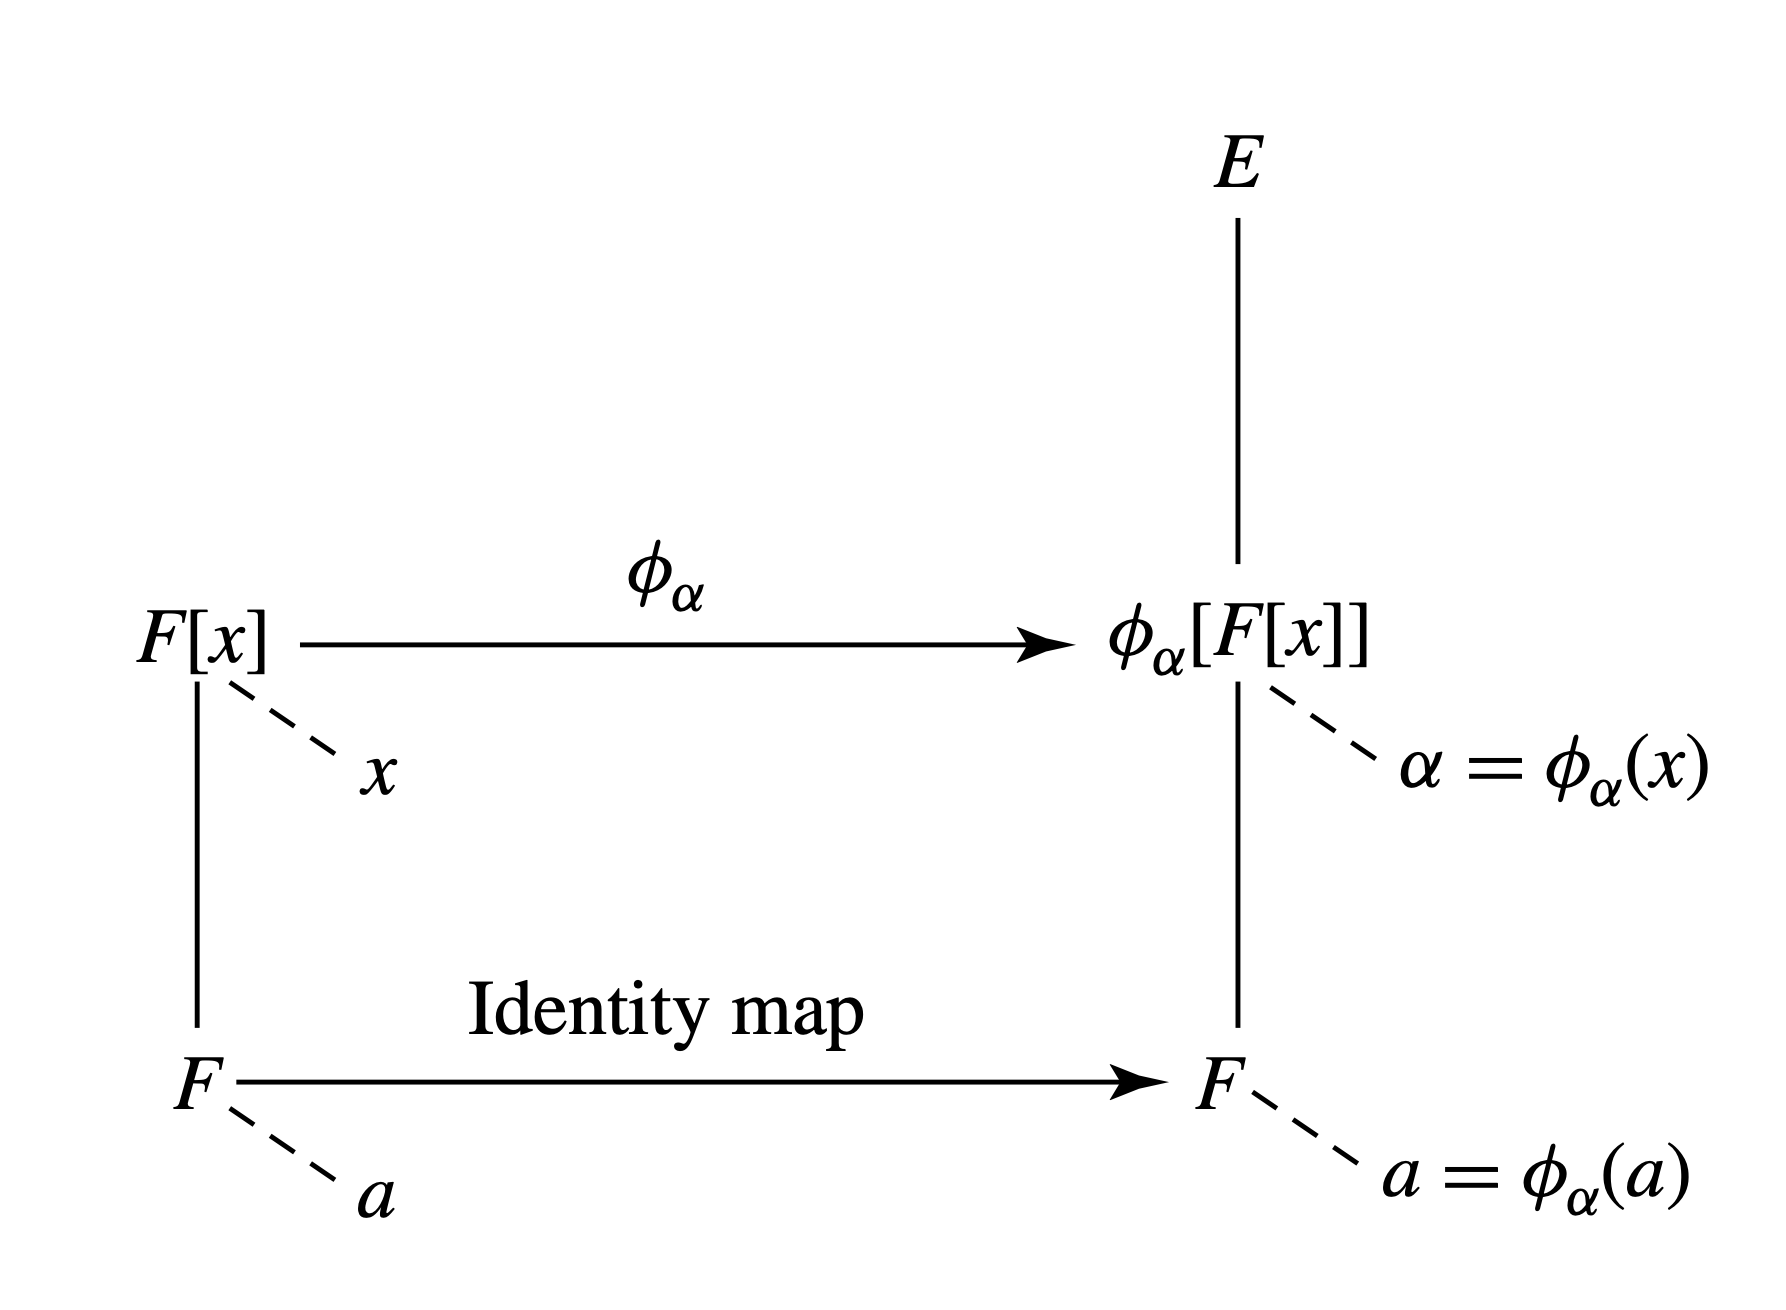
\includegraphics[width=0.5\linewidth]{Screenshot 2023-11-27 at 12.39.20 AM.png}
    \caption{hi}
    \label{fig:enter-label}
\end{figure}

\end{Def}
\begin{note}
    Important things to notice: Evaluation map is a ring homomorphism. 
    \\ $\phi: F[x] \rightarrow F$ as $\phi(p(x)) = p(a)$
    \\Detailed proof below. but here is another proof that after group homomorphism we only need to check it is multiplicative on monomials:
    
\textit{    \href{https://math.stackexchange.com/questions/3825249/showing-in-multiplicative-property-of-ring-homomorphism-in-proof-that-evaluation}{monomials}}
\textit{    \href{https://math.stackexchange.com/questions/935877/how-to-prove-that-the-evaluation-map-is-a-ring-homomorphism}{original proof}}

\end{note}
\begin{Proof}
    Lemma:
    \\ $\phi$ is a ring homomorphism if E is commutative.
    \\ Proof: 
\\ 1) Group Homomoprhism:
Take $\phi (f(x) + g(x))(\beta)$ and WTS it equals $\phi (f(x)) + \phi (g(x))(\beta)$. 
\\ f(x) = $\sum ai x^i$ g(x) =$\sum bj x^j$ 
\\ $\phi (f(x) + g(x))(\beta)$ = $\phi(\sum (ai+bi)x^i)$ if we assume i = max(i,j). 
\\$\phi(\sum (ai+bi)x^i)$ = $\sum (ai+bi) \beta^i$ = $\sum ai\beta^i$ +  $\sum bi\beta^i$ = $\phi (f(x)) + \phi (g(x))(\beta)$. 

2) Ring Homomorphism:
By similar argument, $f(x)g(x) = \sum_k (\sum_{i+k=k} aibj) x^k$
Evaluate x at $\beta$ to get $\phi$. 
\\ $\phi(f(x)(\beta) = \sum ai\beta^i$, $\phi(g(x)(\beta) = \sum bj\beta^j$.
Equals when it is commutative. 
\end{Proof}

\begin{theorem}
    Let E be a field and let F be a subfield of it.
    \\For any $a \in E$ the map $ev_\alpha =  \hat{ev_a} \circ \phi$
    \\ $\hat{ev_a} : F[x] \rightarrow E, \sum aix^i \mapsto \sum ai\alpha^i$ is a ring homomorphism. 
\end{theorem}

\begin{note}
    Let F be a field. In general, the map $\phi: F[x] \rightarrow Map(F,F) $ is not injective, when $char(F) \neq 0$.
   \\ Consider $char (F) = p \Leftrightarrow \Z_p $:
   Consider $f(x) = x - x^p \in F_p[x]$
   \\By FLT:  $f(a) = a - a^p = 0 \in F_p = Z_p$ Then the kernel is not trivial, thus not injective. 
\end{note}


\begin{Example}
About field construction
    Consider $\Q \subseteq \R$, $\pi \in \R  \backslash \Q$ 
    \\ $ev_\pi: \Q[x] \rightarrow \R$ is an injective homomorphism. 
    i.e. $\pi$ is a transendental number s.t. $f(\pi) = 0$ iff all coefficients are zero, ker($ev_\pi$) = $\emptyset$
    \\ $ev_\pi(\Q[x]) = \{ \sum_{i=0}^n ai \pi^i \mid ai \in \Q, n\in \Z^+\}$ is a subring (subdomain) of $\R$ which is isomorphic to $\Q[x]$
\end{Example}
\begin{note}
    $\Q \subseteq \Q[x] \subseteq Frac(\Q[x]) \subseteq \R$
\\ In general, Consider $\alpha \in E\backslash F$ which $\alpha \notin F$.
\\For any evaluation map: $ev_\alpha: F[x] \rightarrow E$, $F[x] \cong ev_\alpha(F(x))\subseteq E$.
\\ The transedental extentions being isomorphic to F[x] as follows:
\textit{\href{https://math.stackexchange.com/questions/1337221/transcendental-extensions-f-alpha-isomorphic-to-fx}{proof on bijection, also going to do later}}
\\ Then $F \subseteq F[x] \subseteq Frac(ev_\alpha F(x)) \subseteq E$.
\end{note}
\begin{Example}
    Consider $\R \subseteq \C$. $i \in \C \backslash \R$.
    $ev_i: \R[x] \rightarrow \C$ is not injective. (Because 1) we know that the evaluation map is homomorphism 2) the kernel is not empty)
    $ev_i(x^2+1) = 0$ then i is an algebraic number over $\R$.
    \\But $ev_i$ is surjective since any $a+bi \in \C $, $a,b \in \R$
    \\ $a + bi = ev_i(a+bx)$ by Fundamental theorem of ring homomorphism:
    $\R[x] / ker(ev_i) \cong \C$ (which is the image of $ev_i$, and is $\Z \times \Z_i$)
    \\$ker(ev_i):= \{f(x)\in \R[x] \mid f(i) = 0\} = (x^2+1)$ the ideal generated by $x^2+1$. Such $\R[x]/(x^2+1)$ is the algebraic construction of the complex field.  
\end{Example}


\begin{theorem}
    If D is an integral domain, then $D[x]$ is also an integral domain. For this case, $deg(f*g) = deg(f) + deg(g)$, $f,g\neq 0, \in D[x]$
\end{theorem}

\begin{Proof}
    We already know that $D[x]$ is a commutative unital ring. Only need to show that $D[x]$ has no zero divisor. 
    \\Take $f(x) = \sum a_ix^i$, $g(x) = \sum b_jx^j$ with $f(x) g(x) = 0$
    Show when $f(x) \neq 0$, $g(x) = 0$, etc,.
\end{Proof}
\begin{Example}
    Let D be an integral domain. What is $(D[x])^\times $ i.e. units of D[x]? 
    \\Answer: $(D[x])^\times = D^\times$. f(x) * g(x) = 1 $\Rightarrow$ deg(f) + deg(g) = 0 $\Rightarrow$ deg(f) = 0 = deg(g) only constant terms. 
    \\e.g. $(\Z[x])^\times = \{\pm 1\}$
\end{Example}
\begin{note}
    In general, for $f,g \in \R[x], f\neq 0, g\neq 0$: $deg(fg) \leq deg(f) + deg(g)$
    \\ i.e. $\Z_6 $ $deg(3x(2x+1)) = 1 < deg(3x) + deg(2x+1)$ But when $\Z_p$ it is an integral domain  $deg(f*g) = deg(f) + deg(g)$.
\end{note}
\newpage





\subsection{Section 23: Factorization of Polynomials over a Field}
Let F be a field. Then F[x] is an integral domain.
\begin{theorem}
\textbf{Division Algorithm for F[x]:}
    F[x] statisfies division algorithm:
    \\ Given any $f(x) = a_0 + a_1 x +...+ a_nx^m$,  
    $g(x) = a_0 + a_1 x +...+ a_nx^n$
    \\ there exist unique q(x), r(x) $\in F[x]$ s.t. f(x) = q(x)g(x) + r(x) with r(x) = 0 or $deg(r(x)) < deg(g(x)) = n$
\end{theorem}

\begin{Proof}
    We first show the existence:
    \\ If $deg f < deg g$, we write $f(x) = g(x)* 0 + f(x)$ with q(x) = 0, f(x) = r(x)
    Then we discuss the cases: 
    \\$deg f< deg g$ then we are done by taking $q(x) = 0, r(x) = f(x)$
    \\ Otherwise, we show by induction.
Then show the uniquess: 
Prove by contradiction:
\\ Assume $f(x) = q_1(x)g(x) + r_1(x) = q_2(x)g(x)+r_2(x)$ 
\\Then $r_1(x) - r_2(x) = (q_2(x)-q_1(x))g(x)$.
\\If $q_2(x)-q_1(x)\neq 0$, deg(RHS) = deg($q_2(x)-q_1(x)$) + deg(g(x))$\geq $ deg(g(x)) =n
\\deg(LHS)$ < n.$
Contradiction. 
\end{Proof}
\begin{Example}
    $f(x) = x^4 - 3x^3 + 2x^3+4x -1$, $g(x) = x^2 - 2x + 3$ in F5[x].
    we can use long division to get $q(x) = x^2 - x-3$, $r(x) = x + 3$.
\end{Example}
\begin{theorem}
    \textbf{cor1:} For any $f(x) \in F(x)$ where F is a field, an element $a \in F$ is a zero of f(x) i.e. f(a) = 0 iff $f(x) = (x-a)g(x)$ for some $g(x) \in F[x]$
    \\\textbf{cor2:} Assume $f(x) \in F[x]$, $f(x) \neq 0$ and $deg(f) = n$. Then f has at most n zeros in F.
\end{theorem}

\begin{Proof}
    \begin{enumerate}
        \item Cor1:
        \\$\Leftarrow$ obvious.

$\Rightarrow$ To show that if $a$ is a zero of $f(x)$ then we have $f(x) = (x-a)g(x)$, we notice that by division algorithm, our $f(x) = q(x)g(x) + r(x)$ thus WTS $r(x) = 0$. Here, our $g(x) = (x-a)$, then we conclude that $deg r < 1, deg r = 0$. Thus $r(x)$ is a constant polynomial, denoted by r. 
\\ When $a$ is a zero of $f(x)$, $f(a) = (a-a)q(a) + r$ thus $r = 0$
        \item Cor2: Using induction.
    \end{enumerate}
\end{Proof}
\begin{Example}
    Use the above cor2: we can show that any finite subgroup of $(F*, \cdot)$ is cyclic where F is a field. In particular, for any finite field, $(F*, \cdot)$ is cyclic. 
\end{Example}


\begin{Def}
    A non-constant polynomial $f(x) \in F[x]$ is called irreducible over F if f(x) can NOT be written as $g(x)h(x)$ with $g, h \in F[x]$, $deg(g) < deg(f)$, $deg(h) < deg(f)$ otherwise f is called reducible over F. 
\end{Def}
\begin{Example}
    $x^2+1 $ is irreducible over R, but reducible over C.
\end{Example}
\begin{Example}
    $x^2-2$ is irreducible over Q, but reducible over R. 
\end{Example}
\begin{note}
    $f(x) \in F[x]$ and non-constant, f is irreducible over F $\Leftrightarrow$ When f(x) = g(x)h(x) for $g, h \in F[x]$ then must be g or h is a unit (a constant).\textbf{ (A unit in F[x] is nonzero constant polynomial in F[x], which are units in F)}
    
\end{note}

\begin{theorem}
    For any $f(x) \in F[x]$ with deg(f) = 2 or 3, f is irreducible over F iff f has no zero in F. 
\end{theorem}
\begin{note}
For degree 2 or 3:If f(x)has a root in F, it can be factored into linear factors (degree 1), proving it's reducible. If f(x) has no root in 
F, it can't be factored into lower degree polynomials, so it's irreducible.
\\For higher degrees (4 or more):The absence of a root in F doesn't guarantee irreducibility. A polynomial of degree 4 or higher might not have roots in F but could still be factored into irreducible polynomials of lower degree (greater than 1), making it reducible.
\end{note}
\begin{Proof}
    We show that "f is reducible over F iff f has zero in F."
   basically expand the above idea. 
\end{Proof}

\begin{theorem}
    Check whether it is irreducible over$\Q$ is the same as check whether it is irreducible over $\Z$
\end{theorem}

\begin{theorem}
    Eisenstein Criterion:
\\ Let $p \in \Z$ that is a prime number. $f(x) = a_nx^n + ...+a_1x + a_0$ which $a_n \neq 0$ mod p, $a \equiv 0$ mod p for $i<n$, and $a_0 \neq 0$ mod $p^2$. Then f(x) is irreducible over $\Q$

\end{theorem}

\begin{Proof}
    Basic Idea: We WTS that it is irreducible over $\Z.$ And we write $f(x) = (b_rx^r + ...+ b_0)(c_sx^s +....+c_0)$ Then we want to follow the criterion in the theorem and try to figure out a contradiction. 
\end{Proof}

\begin{note}
    Cor: For any prime number p:
    \\ $1+x+x^2+...+x^{p-1} =: \Phi_p(x)$ is irreducible over $\Q$. 
\end{note}

\begin{theorem}
    F[x] is UFD = Unique factorization Domain. 
    \\ Any non-constant $f(x)\in F[x]$ can be factored in $F[x]$ into a product of irreducible polynomials.
    The way is unique except for order and for unit factors in F. 
\end{theorem}
\newpage

\subsection{Section 26: Fundamental theorem of ring homomorphism}
\begin{Def}
    A map: $\phi R \rightarrow R'$ for rings R, R' is a ring homomorphism, if:
    \\$\phi(a+b) = \phi(a) + \phi(b)$
    \\$\phi(ab) = \phi(a)  \phi(b)$
    
\end{Def}

\begin{theorem}
    For a ring homomoprhism: $\phi: R \rightarrow R'$
    \begin{enumerate}
        \item For any subring S of R, $\phi(s)$  is a subring of R'.
        \item For any subring S' of R', $\phi(s')$ is a subring of R.
        \item $\phi(1)$ is the unity of $\phi(R)$ if 1 is the unity of R. 
    \end{enumerate}

\end{theorem}

\begin{note}
        It is possible that $\phi: R \rightarrow R'$ is ring homomorphism, R is unital but R' is not.
        \\e.g. R = $\Z$, R = $\Z \times 3\Z$.
        \\ $\phi: \Z \rightarrow \Z \times 3\Z$
\end{note}


\begin{Def}
    Let $\phi: R \rightarrow R'$ be a  ring homomorphism. s.t. ker$\phi = \phi^{-1}(0)$
\end{Def}

\begin{Example}
    The modulo n map: $\phi: \Z \rightarrow \Z_n$ is a ring homomorphism with ker($\phi$) = $n\Z$
\end{Example}

\begin{Def}
    Let R be a ring. An additive subgroup I of R is called an ideal of R if:
    \\ $aI\subseteq I$, $Ia \subseteq I$ for all $a \in R$
\end{Def}
\begin{note}
    (1) An ideal is a subring of R since for any $a,b \in I$:  $ab \in aI \subseteq I$
    \\(2) {0} is always an ideal called trivial ideal of R.
\end{note}
\begin{theorem}
    Let $\phi: R \rightarrow R'$ be a ring homomorphism. Then the kernel is an ideal of R.
\end{theorem}
\begin{Proof}
    Kernel is a subgroup shown before. Now we check for any $r\in R$, we take $k \in ker(\phi)$. WTS $rk \in ker(\phi)$.
    $\phi(rk) = \phi(r) \phi(k) = 0$ Thus $rk \in ker(\phi)$.
\end{Proof}

\begin{note}
    Group $\leftrightarrow$ Ring, Normal subgroup $\leftrightarrow$ ideal,
    Quotient Group $\leftrightarrow$ Quotient Ring.
\end{note}

\begin{theorem}
    Let R be a ring and I be an ideal of it.
    Then the quotient group R/I of $(R, +)$ has a natural ring structure induced from the ring R.
    \\ The quotient map $\phi: R \rightarrow R/I$ is a surjective ring homomorphism with ker($\phi$) = I.
\end{theorem}

\begin{Proof}
\hfill
\\Notice binary operations on R/I: $(a+I)(b+I) = ab + I$ and $(a+I)+(b+I) = (a+b) + I$
\begin{enumerate}
 \item We check if multiplication is well defined on R/I. Just as the construction in quotient groups, we define:
\\ 
\textbf{$(a+I)(b+I) = ab + I$ }
we check by different representation of a and b, which $a+I =a'+I$, $b+I = b'+I$
....details unfinished for next week 
Then we checked it is a ring.
\item Then we check the quotient map $\phi: R \rightarrow R'$ is a ring homomorphism. We know it is a group homomorphism and surjective by construction, then we know that:
By our construction: $\phi(ab) = ab + I = (a+I)(b+I) = \phi(a) \phi(b)$ with kernel = I.

\end{enumerate}


\end{Proof}


\begin{theorem}
    Fundamental theorem of ring homomorphism:
    \\Let $\phi:R \rightarrow R'$ be a ring homomorphism with kernel k. 
    \\Then (1) $\phi(k)$ is a subring of R'
    \\(2) K is an ideal of R.
    \\(3) The quotient ring R/k is ring isomorphic to $\phi [R]$ via the map:
    \\$\bar{\phi}: R/k \rightarrow \phi(R)$
    \\$\bar{\phi}: a+I \mapsto \phi(a)$
\end{theorem}\

\begin{Proof}
    We did that $\phi(R)$ is a subring of R' and the quotient map$\pi: R \rightarrow R/I$ is a surjective ring homomorphism with kernel = I.
    \\Now we want to show that $\hat{\phi}: R/K \rightarrow \phi(R)$ which is $a+I \mapsto \phi(a)$ is a ring isomorphism.
    \\We check that $\hat{\phi}$ is well defined:
    Idea: Consider different representative $a'+k = a+k $ but  $\hat{\phi}(a'+K) = \hat{\phi}(a+K)$
    \\ Then we already know that $\hat{\phi}$ is a group isomorphism. Only need to check it is a ring homomorphism.
\end{Proof}

\begin{Example}
    Definition for nilradical:

 \\ N:= $\{ a \in R \mid a^n = 0$ for some $n \in \Z^+$\} is an ideal of R.
\end{Example}

\begin{Example}
    Definition for radical:
     \\ $\sqrt{N}$ := $\{ a \in R \mid a^n = N$ for some $n \in \Z^+$\} is an ideal of R.
\end{Example}

\begin{Example}
    What is the nilradical of R/N for an ideal N in a commutative ring R? 
    \\ Consider $(a+N)^n = a^n +N = 0 + N$
    \\Thus $a^n \in N, a\in \sqrt(N)$ that $a+N$ is in the nilradical of R/N.
\end{Example}

\newpage



% ------------------------------------------------------------------------------




\subsection{Section 27:Prime and Maximal ideals}
\begin{note}
    Some difference between Normal subgroup and Ideal:
    \\Ideal has the property that $Ia \subseteq I$ while normal subrgoup only is that $gh = hg$
    \\If we are considering $\Z$, we get normal subgroup by addition, but get ideal by considering closure under multiplication with ring elements. 
    \\\textbf{Ideal is ring.} closed under addition, and closed under multiplication with Ring Elements.
    \\Although \textbf{the quotient ring is a ring.}
\end{note}

\begin{Def}
    A \textbf{maximal ideal} of a ring R is an ideal M different from R such that there is no proper ideal N of R properly containing M.
\end{Def}
\begin{Def}
    An ideal$ N \neq R $ in a commutative ring R \textbf{is a prime ideal} if $ab \in N$ implies that either $a\in N $ or $b \in N$ for $a,b\in R$.
    \\Note that $\{0\}$ is a prime ideal in $\Z$, and indeed, in any integral domain. 
\end{Def}

\begin{note}
    All nontrivial ring has 2 ideals: itself and $\{0\}$.
    \\Also, for a unital ring, if an ideal I contains a unit, then I = R.
    \\We can show that by proof: $a \in R$ write $a = u(u^{-1}a) \in I(u^{-1}a) \subseteq R$
    
\end{note}
\begin{Example}
    When n is prime, $\Z/n\Z \cong \Z_n$ is a field.
    \\ When n is not prime,  $\Z/n\Z \cong \Z_n$ is not an integral domain.
    \\(n) is maximal ideal and prime ideal when n is prime. 
\end{Example}
\begin{theorem}
    A field contains no proper nontrivial ideals. 
\end{theorem}
\begin{Proof}
    Any improper nontrivial ideal in a field must contain unit element, and then is the field itself. 
\end{Proof}
\begin{theorem}
    If I, J are two ideals of ring R, then $I \cap J$ and $I+J = \{ a+b \mid a \in I, b \in J \}$ are ideals of R. 
\end{theorem}
\begin{theorem}
    Let R be a commutative untial ring, and I is an ideal of R.
    \begin{itemize}
        \item I is a prime ideal $\Leftrightarrow$ R/I is an integral domain.
        \item I is a maximal ideal $\Leftrightarrow$ R/I is a field.
        
    \end{itemize}
    Cor: A maximal ideal in a commutative unital ring must be a prime ideal since a field must be an integral domain. 
\end{theorem}
\begin{Proof}
   1) "$\Rightarrow$"I is a prime ideal: we want to show that $R/I$ is an integral domain. Only need to show that $R/I$ has no divisor of zero.
   Consider element in $R/I$ which $(a+I)(b+I) = 0 + I \Rightarrow (ab) + I$  By how we take coset: $ab \in I$. Since I is a prime ideal, thus either $a \in I $ or $b \in I \Rightarrow a + I \in I $ or $b + I \in I$. Thus it is an integral domain.
\\ 1) "$\Leftarrow$" If $R/I$ is an integral domain, then $(a+I)(b+I) = 0 + I \Rightarrow $ either $a+I = I \Rightarrow a \in I$ or $b + I = I\Rightarrow b \in I $. Consider $ab \in I$ thus we either have $a \in I $ or $b \in I$.
\\2) "$\Rightarrow$" I is a maximal ideal, to show that $R/I$ is a field, we show any $a + I$ is a unit. Consider element $a \notin I$, and the any $(a) := {ax| x \in R}$ is an ideal. By previous theorem, $I + (a)$ is an ideal in R. We know that $I \subset I +(a)$ but I is the maximal ideal, thus $I + (a) = R$. Thus $ I + (a)$ contains unity 1.  Then we consider $(a+I)(x+I) = ax + I = I + (a)$ which contains 1. So there exists $x \in R$ s.t. $(a+I)(x+I) = 1$ and $a + I$ is  a unit.
\\2) "$\Leftarrow$" If $R/I$ is a field, we want to show that $I$ is the maximal ideal. $a + I \in R/I$ is a unit, thus $(a+I)(x+I) = 1 = ax + I$ for some $x\in R$. We claim that $(a) = ax$ is the smallest ideal we can get, thus anything strictly bigger than $I$ must contain unity, and thus $ = R$. Then we show that $I$ is the maximal ideal.

\end{Proof}
\begin{note}
    If I1 is an ideal of A, I2 is an ideal of B, then $I1 \times I2$is an ideal of $A \times B$
\end{note}
\begin{theorem}
    If R is a ring with unity and N is an ideal of R containing a unit, then N = R.
\end{theorem}
\begin{Proof}
If $1 \in I$ then I = R since $r1 = r$ for all $r \in R$. If N contains a unit element, then $r*u \in I$ that u is the unit element in ideal. If we take $r = u^{-1}$, then $1 \in I$, then N = R.
\end{Proof}
\textbf{Ideal Structure of F[x]:}
\begin{Def}
    If R is a commutative ring with unity and $a \in R$, the ideal $\{ra \mid r \in R\}$  of all multiples of a is the \textbf{principal ideal generated by a} and denoted by $<a>$. An ideal N of R is \textbf{a principal ideal} if $N = <a>$ for some $a \in R$.
\end{Def}
\begin{Def}
    An integral domain D is called a principal ideal domain (PID) if every ideal of D is a principal ideal.
\end{Def}
\begin{theorem}
    F[x] with F is a field is a PID. 
    \\? In fact, any integral domain with division algorithm is a PID.
   \\ $\Z$ is a PID.
\end{theorem}
\begin{Proof}
    To show that $F[x]$ is a PID, we show all ideals are principal. 
    \\ Take $I \in F[x]$ that is the ideal.
    \\ We want to show that all $ f(x) \in I$ is generated by some polynomial $p(x)$.
    \\ Thus we take $p(x)$ to be the polynomial with min degree. 
    \\If $I = {0}$, then I = $<0>$. We consider when $p(x)$ has degree 0, then $p(x)$ is a unit, and by previous theorem, if our ideal contains unit, then $I = F[x]$, it is true that all $f(x) \in I$.

    \\Now, take $p(x)$ to be the polynomial that at least have a degree 1. Because our $F[x]$ has division algorithm, we can show that $f(x) = q(x)p(x) + r(x)$ which $r(x)$ has degree less than deg(p(x)) or $r(x) = 0$. Thus our job is to show that $r(x) = 0 $ then we are done.
    \\ Notice that $f(x), p(x) \in I$, thus $q(x)g(x) \in I$, $f(x) - q(x)g(x) = r(x) \in I.$ We define $p(x)$ to have the minimum degree and $p(x)>= 1$ so $r(x)$ can only be 0. 
\end{Proof}

\begin{Example}
    Consider the ideal $I = (x) + (3) : = {x, 3, x+3, 2x+3, ....}$
    \\ I is a principle ideal in $Q[x]$, which $Q[x]$ is PID, but not a principle ideal in $Z[x]$.
    Consider $(2x+3)/(x+3) \notin Z[x]$ but $\in Q[x]$ which the latter has division algorithm.
    
\end{Example}


\begin{theorem}
    In a PID, any nontrivial prime ideal is a maximal ideal.
\end{theorem}

\begin{Proof}
    Consider $P= (p) \in D$ that D is a PID, and P is a prime ideal. WTS P is a maximal ideal.
    \\Take ideal $I = (q)$ that $P\subset I \subseteq D$ We want to show that I = D.
   \\ Consider that take $p \in P$, $ p\subset I = (q)$ thus $p \in (q)$. we can write $p = a \cdot q$ for some $a \in D$. Then notice that P is a prime ideal. Thus if $p = aq \in P$, either have $a \in P$ or $q \in P$. If $q \in P$, then I is not strictly larger than P, contradict our assumption, thus $a \in P = (p)$.  We can write $a = bp | b \in D$.
   \\Then: $p = a \cdot q = bp \cdot q$  $\Rightarrow 1= bq.$ Thus we can show that $q \in (q) = I$ is a unit, thus I = D.  
   
\end{Proof}

\begin{Example}
    Consider $F[x]$ which F is a field, then $F[x]$ has divison algorithm $\Rightarrow$ $F[x]$ is PID. $\Rightarrow$ In $F[x]$ non prime ideal is maximal ideal.
    \\ When $f(x) \neq 0, (f(x))$ is maximal $\Leftrightarrow f(x)$ is irreducible.
\end{Example}

\begin{Proof}
When $f(x) \neq 0$:
  1)   WTS that when $(f(x))$ is maximal $\Rightarrow$ $f(x)$ is irreducible. 
    \\ Assume by contradiction, we can factorize $f(x) = p(x)q(x)$ \\ s.t.deg $p(x)$ and deg $q(x) <$ deg $f(x)$. 
    \\ Thus since all maximal ideals are prime ideal, $p(x) \in (f(x))$ or $q(x) \in (f(x))$. Then we either $p(x)$ or $q(x)$ will have $f(x)$ as a factor, that then has degree $>=$ degree of $f(x)$.
    \\Thus, it is not possible to have $f(x) = p(x)q(x)$ s.t.deg $p(x)$ and deg $q(x) <$ deg $f(x)$. 
\\
2)  WTS that when $f(x)$ is irreducible $\Rightarrow$ $(f(x))$ is maximal ideal. We want to show that assume we have ideal N that $(f(x)) \subset N \subset F[x]$ such N must be F[x]. Then by that $F[x]$ is PID, we know $N$ can be written as $N = (g(x))$. 
\\Since $(f(x)) \subset (N = (g(x)) )\Rightarrow $
for $f(x) \in (f(x))$, $f(x) \in (g(x)) \Rightarrow$, $f(x) = q(x)g(x)$, but since we know that $f(x)$ is irreducible, either $q(x)$ or $g(x)$ has degree 0, we know that $g(x)$ has a degree 0 $\Rightarrow g(x)$ is a unit. Thus $(g(x))= N = F[x]$.
\\Otherwise, $q(x)$ has degree 0 and a unit. $(f(x)) = F[x]$. Still contradiction. Thus $(f(x))$ is maximal if it is irredcible. 
\end{Proof}

\begin{theorem}
    A PID is a UFD.
\\ Let $p(x)$ be an irreducible polynomial in $F[x]$. If $p(x)$ divides $r(x)s(x)$ for$r(x), s(x) \in F[x]$, then either $p(x)$ divides $r(x)$ or $p(x)$ divides $s(x)$.
\end{theorem}

\begin{Proof}
    Suppose $p(x)$ divides $r(x)s(x)$, Then $r(x)s(x)\in <p(x)>$, which is maximal. Then $<p(x)>$ is prime ideal. Hence $r(x)s(x)\in <p(x)> \Rightarrow $ implies $r(x) \in <p(x)>$ or $s(x) \in <p(x)>$ giving $p(x)$ divides $r(x)$ and also $s(x)$. 
\end{Proof}

\newpage
\subsection{Section 29: Extension Fields}
\begin{note}
    Consider to find the zero of $f(x) = x^2 + 1 \in \R[x] $ then we extend to complex field.
\end{note}
\begin{Def}
    A field extension if a pair of fields $F\subseteq E$ so that the operations of F are the restriction of the operations of E, i.e. F is a subfield of E. E is called an extension of F.
\end{Def}

\begin{theorem}
    Kronecker's theorem:
    Let F be a field. $f(x) \in F[x]$, $f(x)$ is not constant polynomial. Then there must be an extension field E of F and an $\alpha \in E$ such that $f(\alpha) = 0$.
\end{theorem}
\begin{Proof}
    We can explicitly construct such an extension E as follows:
\\ $f(x) = p_1(x)p_2(x)p_3(x)...p_n(x)$ each $p_i$ is irreducible, as $f(x)\in F[x]$. $(p_1(x))$is the maximal ideal $\Rightarrow$ $F[x]/(p_1(x))$ =: E is a field. 
\\ \textbf{(1) E is an extension field of F:} construct $\phi: F \rightarrow E$, $a \mapsto a + (p_1(x))$ We want to show such map is an injective map, thus it make sense to have $F\subseteq E$. To show such map is injective, we can either directly  show $\phi(a) = \phi(b)\Rightarrow a = b$ or show that it is a homomorphism then kernel is empty.
\\ We can directly show that $\phi(a) = \phi(b)\Rightarrow a = b$ by considering
\\$\phi(a) = a + (p_i(x)) = b + (p_i(x)) =\phi(b)\Rightarrow  a - b \in (p_i(x))$
\\ Thus we know that $a - b$ is a multiple of $(p_i(x))$, but the latter has a degree $\geq 1$ by construction. $a - b \in F$ either $a - b$ is a constant polynomial of degree 0, or is the zero polynomial. But if it has degree 0, it will contradict the fact that $(p_i(x))$ at least has degree 1 and it can only be the zero polynomial. Thus a = b.
\\IF we want do the other way: we know that is it a homomophism considering
\\$Map : F\rightarrow F[x] \rightarrow F[x]/(p_i(x))$. It is the composition of two homomorphisms, the first is homomorphism by the natural induction map is injective homomorphism, the second is true by the quotient map is a surjective homomorhism. Then now we consider the kernel of such map: $ker(\phi) = \{a \in F \mid a + (p_1(x)) = 0 + (p_1(x))\}$ Following the previous argument, $a \in (p_1(x)$ thus $a = 0$ Thus $\phi$ is injective. 
\end{Proof}
\begin{Proof}
    Continue.


 \\\textbf{(2) $f(x) \in F[x] \subseteq E[x]= F[x]/(f(x))$ has zero for f(x) in E.}
 Consider any f(x) = p(x) in the following arguments:
 Let us set $\alpha = x + (p(x))$ is a solution as well as an element in the quotient field.
 \\Thus consider the evaluation homomorphism $\phi_a : F[x] \rightarrow E$. If $p(x) = a_0+a_1x+...+a_nx^n$ where $a_i \in F$ then we have: \\$\phi_a(p(x)) = p(\alpha) = a_0 + a_1(x+(p(x))) +  ... + a_n(x+(p(x)))^n$ in $E = F[x]/ (p(x))$.
 \\We take our x as the representative of the coset $\alpha = x + (p(x))$. 
 \\For example $a_1(x+(p(x))) = a_1x + (p(x))$ therefore:
 \\ $p(\alpha) = a_0 + a_1(x+(p(x))) +  ... + a_n(x+(p(x)))^n = (a_0+ a_1x + a_2x^2 + ..a_nx^n) + (p(x))$ 
 \\$
 = p(x) + (p(x)) = (p(x)) = 0 $ in E = $F[x]/(p(x))$ Thus we can conclude that $p(\alpha) = 0 $ and it is has zero in E.
 
 
\end{Proof}

\begin{Example}
    Take our $F = \R$. Let $f(x)=x^2+1$ which has no zero over $\R$ and is thus is irreducible over R, and $(f(x))$ is a maximal ideal in R. 
    \\WTS that if we take: 
    $\R/(f(x))$, then this is a zero for $f(x)$ in quotient field that is:
    $\alpha = x + (f(x)) = x+ (x^2+1)$
   \\ Then consider the evalution of $f(x)$ in E at $\alpha$, consider $I = x^2 +1$:
   \\ $f(\alpha) = a^2 + 1 \in F \Rightarrow (x+I)^2 + 1)\in E$
   \\ $ = (x+I)^2 + =1 = (x^2 + I) + 1 = (x^2+1) + I  = 0 + I $
\end{Example}

\begin{Example}
    $F = \Q$, $f(x) = x^4 -5x^2 + 6 = (x^2 -2)(x^2 -3)$
    \\ Then $E1:= \Q[x]/(x^2-2)$, 
    $E2:= \Q[x]/(x^2-3)$
\end{Example}
\begin{Def}
    Let $F \subseteq E$ be a field extension. An element $\alpha \in E$ is called algebraic over F, if there is some $f(x) \in F[x]$ s.t. $f(\alpha) = 0$. Otherwise, $\alpha$ is called transcendental over F.  
\end{Def}

\begin{Example}
\\ 1) $\R \subseteq \C$ i is algebraic over R. 
\\ 2) $\Q \subseteq \R$ $\sqrt{3}$ is algebraic over $\Q$.
\\ 3) $\pi, e$ are transecendental over $\Q$ but they are algebraic over $\R$ like $(x - \pi)\in \R[x] $.
\end{Example}

\begin{theorem}
    Let $F \subseteq E$ be a field extension, $\alpha 
    \in E$ is algebraic over F.
\\ Then $ker(eV_\alpha) = \{ f(x) \in F[x] \mid eV_\alpha(f) = 0\}$ (Note that this counts for \textbf{ALL} $f(x)$ that take $\alpha$ as a zero) is a principal ideal of F[x], which is generated by some irreducible polynomial $p(x) \in F[x]$ with degree $\geq 1$. This degree is independent of the choices of generators of $ker(eV_\alpha)$ and is defined as the degree of $\alpha$ over F, written as $deg(\alpha;F)$.
\end{theorem}

\begin{note}
    There is a few things to note.
\\ 1) Consider the evaluation map: $eV_\alpha: F[x] \rightarrow E$ this is a ring homomorphism. And thus kernel is an ideal lives in $F[x]$. Since it is a PID, we know the kernal is a principle ideal. 
\\ 2) It is generated by irreducible polynomial $p(x)$ with degree $\geq 1$ because when we show all ideals are principle in proving it is PID, we take our $p(x)$ to be the ideal with min degree.
And if $p(x)$ is reducible, then there exists other polynimal with degree less than deg $ p(x)$.
Here just consider $ker(eV_\alpha) = I$, and all polynomials $f(\alpha) = 0 \in I$, thus $f(x) = p(x) q(x) = (p(x))$ s.t. it is irreducible.
\\3) Degree is independent of the choice of generator because of the same reason, as it is the minimal degree.
\\4) An example of this would be consider $\alpha = \sqrt{1+ \sqrt{3}}$ that is algebraic over $\Q$ with $f(x) = x^4 -2x^3 -2 \in \Q[x]$, $f(\alpha) = 0$ in E. And our polynomial has degree 4, so $p(x) =x^4 -2x^3 -2 $ but there are other polynomials can be in $ker(eV_\alpha)$ such as $2(x^4 -2x^3 -2)$ or anything $(x^4 -2x^3 -2)$.
\end{note}

The alternative statement of the theorem in textbook is theorem 29.13.

\begin{theorem}
Let E be an extension field of F, and let $\alpha \in E$ where $\alpha$ is algebraic over F. Then there is an irreducible polynomial $p(x) \in F[x]$ such that $p(\alpha) = 0$. This irreducible polynomial p(x) is uniquely determined up to a constant factor in F and is a polynomial of minimal degree $\geq$1 in $F[x]$ having $\alpha$ as a zero. If $f(\alpha) = 0$ for $f(x) \in F[x]$ with $f(x)\neq 0$ then $p(x)$ divides $f(x)$
    
\end{theorem}

\begin{Proof}
    As $\phi_{\alpha}$ be the evaluation homomorphism of $F[x]$ into E. The kernel is an ideal and must be the principal ideal since we are in $F[x]$, generated by $p(x)\in F[x]$.
    $<p(x)>$ consists precisely the elements of $F[x]$ that has $\alpha$ as a zero. Then $f(\alpha) = 0$ for $f(x) \neq 0$ then $f(x) \in <p(x)>$ so that $p(x)$ divides $f(x)$. Thus $p(x)$ is a polynomial of minimal degree $geq$ 1 having $\alpha$ as a zero, and any other such polynomial of the same degree must be in the form of $a p(x)$ for $a \in F$.
    \\ We are left to show that such $p(x)$ is irreducible. If $p(x) = r(x)s(x)$ were a factorization of $p(x)$ into polynomials of lower degree, then $p(\alpha) = 0$ implies $r(x) = 0$ or $s(x) = 0$ Then they will have a lower degree, that contradicts the fact that we *required* our $p(x)$ is of minimal degree $\geq 1$ such that $p(\alpha) = 0$, contradiction.
\end{Proof}
\begin{Example}
Consider:
\\$(x^2-2) \in \Q[x]$ is irreducible. $(x^2-2) = ker(eV_\sqrt{2})$, deg($\sqrt{2}, \Q$) =2. deg($\sqrt{2}, \R$) =1
\end{Example}
Let $F \subseteq E$ be a field extension. $\alpha \in E$ :
\\ Two cases:
\\(1) $\alpha$ is transecendental over F. 
\\ (1) $\alpha$ is algebraic over F. 

Consider the ring homomoprhism:
$eV_\alpha: F[x] \rightarrow E$.
\\ Case (1) $\Leftrightarrow$ $eV_\alpha$ is injective. In this case, $eV_\a(F[x])$ is a subdomain of E and and its field of fractions is denoted by: $F(\alpha): = Frac(eV_\alpha(F[x]))$ 
\\ This is the tower of fields: $F \subseteq F(\alpha) \subseteq E$
\\Case (2) $\Leftrightarrow$ $eV_\alpha$ is not injective, which the kernel is not trivial but 
\\ $ker(eV_\alpha) = (p(x))$ deg(p(x)) $\geq$ 1.
\\ In this case, $F(\alpha): = F[x]/ ker(eV_\alpha)$. 
\\ Again, the same tower of fields holds as $F \subseteq F(\alpha) \cong eV_\alpha(F[x]) \subseteq E$.
\begin{Def}
    Ab extension field E of a field F is a simple extension of F if E = F($\alpha$) for some $\alpha \in E$.
\end{Def}


\begin{note}
    In book, we have: 
    \\Let $ \phi_\alpha$ be the evaluation homomorphism of F[x] into E.
    \\Case I:
Suppose$\alpha$ is algebraic over F. Then as in Theorem 29.13, the kernel of $\phi_\alpha$ is ⟨irr(α, F)⟩ and by Theorem 27.25, ⟨irr(α, F)⟩ is a maximal ideal of F[x]. Therefore, F[x]/⟨irr(α, F)⟩ is a field and is isomorphic to the image φα[F[x]] in E. This subfield φα[F[x]] of E is then the smallest subfield of E containing F and α. We shall denote this field by F(α).

\\Case II: 
Suppose $\alpha$ is transcendental over F. Then by Theorem 29.12(as the map $\phi_\alpha$ is an injective map since the kernel is empty with image D), $\phi_\alpha$ gives an isomorphism of F[x] with a subdomain D of E. Thus in this case $\phi_\alpha$[F[x]] is not a field but an integral domain that we shall denote by F[$\alpha$]. By Corollary 21.8, E contains a field of quotients of F[$\alpha$], which is thus the smallest subfield of E containing F and $\alpha$. As in Case I, we denote this field by F[$\alpha$].
\end{note}

\begin{theorem}
    Let E be a simple extension F($\alpha$) if a field F, and let $\alpha$ be algebraic over F. Let the degree irr($\alpha$,F) be $n\geq 1$, then every element $\beta$ of E = F($\alpha$) can be uniquely expressed in the form:
    \\ $\beta = b_0+b_1\alpha + ... + b_{n-1}a^{n-1}$ where $b_i$ are in F.
\end{theorem}
\begin{Proof}
    For the usual evaluation homomorphism $\phi_\alpha$, every element of $F(\alpha) = \phi_\alpha[F[x]]$ is of the form $\phi_\alpha(f(x)) = f(\alpha)$, a form polynomial in $\alpha$ with coefficients in F. 
    \\Let  irr($\alpha$, F) = p(x) = $x^n + a_{n-1}x^{n-1} + ... + a_0$
    \\ Then $p(\alpha) = 0$, so 
\\$\alpha^n = -a_{n-1} \alpha ^{n-1}-...-a_0$. This equation in $F(\alpha)$ can be used to express every monomial $\alpha ^m$ for $m \geq n$ in terms of powers of $\alpha$ that are less than n. For example, $\alpha^{n+1} = \alpha \alpha^n = -a_{n-1}\alpha^n - a_{n-2}\alpha^{n-1} - ... - a_0\alpha = -a_{n-1}(-a_{n-1}\alpha^{n-1} - ... - a_0)-a_{n-2}\alpha^{n-1} - ... - a_0\alpha$
\\
\textbf{Unique Representation}: Now, consider any element \(\beta\) in \(F(\alpha)\). Since \(\beta\) is in \(F(\alpha)\), it can be written as a polynomial in \(\alpha\) with coefficients in \(F\). Let's say 
\[
\beta = c_0 + c_1\alpha + c_2\alpha^2 + \ldots + c_m\alpha^m.
\]
If \(m < n\), we are already in the desired form. However, if \(m \geq n\), we use the relation 
\[
\alpha^n = -a_{n-1}\alpha^{n-1} - \ldots - a_0
\]
to express \(\alpha^m\) (for \(m \geq n\)) in terms of powers of \(\alpha\) that are less than \(n\).

By repeatedly applying this process, any power of \(\alpha\) greater than or equal to \(n\) is reduced to a linear combination of \(1, \alpha, \alpha^2, \ldots, \alpha^{n-1}\). Hence, every element \(\beta\) in \(E = F(\alpha)\) can be uniquely expressed as 
\[
\beta = b_0 + b_1\alpha + \ldots + b_{n-1}\alpha^{n-1},
\]
where each \(b_i\) is in \(F\).

\end{Proof}
\begin{Example}
    An example of this is consider $p(x) = x^2 + x + 1 \in \Z_2[x]$ is irreducible over $\Z_2$. By this theorem, we can say that $\Z_2(\alpha)$ has an elements 0 + 0$\alpha$,0 + 1$\alpha$, 1 + 0$\alpha$, 1 + 1$\alpha$.
\\ \textbf{Also WTS the extension $\R[x]/ <x^2+1> \simeq \C$ } Consider $\R(\alpha) = \R[x]/<x^2+1>$ by this theorem, we can know that all elements in $\R(\alpha)$ are in the form of $a + b\alpha$. And $\alpha = x + <x^2+1>$ by construction, $\alpha^2 + 1 = 0$, we see that $\alpha $ plays the role of $i\in \C $ and that $(a+b \alpha) = (a+bi) \in \C$
\end{Example}
\newpage

\subsection{Section 30: Vector Spaces}
\begin{Def}
    Linear space over $\R$ (objective of linear algebra) is a set V with two operations: 
    \\Addition + : $V \times V \rightarrow V$
    \\Scalar multiplication: $\R \times V \rightarrow V$ satisfying the following 10 properties.
    \begin{enumerate}
        \item +: $V \times V \rightarrow V$ is associative.
        \item there is 0 vector so that $0+v=v=v+0$
        \item Every $v \in V$ has $+$ inverse $-v$ so that $v+(-v) = 0 = (-v)+v$
        \item $+$ is commutative
        \item Scalar multiplication $\cdot$ has $\alpha \cdot (\beta \cdot v) = (\alpha\beta) \cdot v$ for $\alpha, \beta \in \R, v\in V$.
        \item $1 \cdot v = v$ for every $v \in V$
        \item Distributive Property:
        $(\alpha + \beta) \cdot V = (\alpha \cdot V) + (\beta \cdot V)$ for $\alpha, \beta \in \R, v\in V$.
        \item Distributive Property: 
        $\alpha \cdot (V+W) = (\alpha \cdot V) + (\alpha \cdot W)$ for $\alpha,  \in \R, V, W\in V$.
    \end{enumerate}
\end{Def}

\begin{Def}
    Let F be a field, a vector space or a linear space over F is an abelian group $(V, +)$ with a scalar multiplication:
    $F\times V \rightarrow V$ with the conditions:
    \begin{enumerate}
        \item Scalar multiplication $\cdot$ has $\alpha \cdot (\beta \cdot v) = (\alpha\beta) \cdot v$ for $\alpha, \beta \in \R, v\in V$. 
        \item $1 \cdot v = v$ for every $v \in V$
        \item Distributive Property:
        $(\alpha + \beta) \cdot V = (\alpha \cdot V) + (\beta \cdot V)$ for $\alpha, \beta \in \R, v\in V$.
        \item Distributive Property: 
        $\alpha \cdot (V+W) = (\alpha \cdot V) + (\alpha \cdot W)$ for $\alpha,  \in \R, V, W\in V$.
    \end{enumerate}
\end{Def}
\begin{Def}
    Let V be a vector space over F. A subspace of C is a subgroup W of V, which is closed under scalar multiplication. We write it as $W\leq V \Rightarrow$ quotient vector space $V/W$. 
\end{Def}
\begin{note}
    We will need to check if the scalar multiplication is well-defined on the quotient space, that is to check : take $v1 + W = v2+ W$ if $k \cdot v1 + W ?= k \cdot v2 + W$ 
    \\ notice that we define $\cdot$ as $k\cdot (v+W) = (k \cdot v) + W$ 
\end{note}
\begin{Example}
Consider two examples:
    \begin{enumerate}
        \item F field. F[x] is a vector space over F, and let I be an ideal of F[x], then I is a subspace of F[x].
        \\It follows $F[x]/I$ is vector space over F,
        \item 
        $F \subseteq E$ is a field extension. Then E is a vector space over F.
        In particular simple extension $F(\alpha)$ is a vector space over F.
    \end{enumerate}
\end{Example}

\begin{note}
    some remarks from linear algebra: 
\\  Linear Independent: consider the set of vectors ${1, v_1,v_2,..., v_n}$ then the solution to $b_0+b_1v_1+b_2v_2...= 0$ is trivial that all $b_i$ = 0. 
\\ Linear Dependent:  there exists $b_i$ such that $b_0+b_1v_1+b_2v_2...= 0$ \textbf{not} all $b_i$ = 0
\end{note}
\begin{theorem}
    In a finite-dimensional vector space, every finite set of vectors spanning the space contains a subset that is a basis.
\end{theorem}
Cor:A finite dim vector space has a finite basis.
\newpage
\begin{theorem}
    Let E be an extension field of F, and let $\alpha \in E$ be algebraic over F. If deg($\alpha$, F) = n, then  F($\alpha$) is an n-dimensional vector space over F with basis $\{1, \alpha, ..., \alpha^{n-1} \}$. Furthermore, every elements $\beta$ of F$(\alpha)$ is algebraic  over F, and deg$(\beta, F)$ $\leq$ deg($\alpha$, F)
\end{theorem}
\begin{note}
    Also, deg($\beta$, F) divides deg($\alpha$, F).
\end{note}
\begin{Proof} To show such:

    \begin{enumerate}
        \item We first show that $F(\alpha)$ is a vector space. By definition, 
        \\$F(\alpha) =F[x]/<irr(\alpha, F[x])>$ By previous theorem, it is the quotient vector space.
        \item We then show that $\{1, \alpha, ..., \alpha^{n-1} \}$ is a basis, and it is a $n$ dim vector space.
        By previous theorem, every element in $F(\alpha)$ can be written as $\beta \in F[x] = c_0+c_1 \alpha + ... + c_{n-1} \alpha ^{n-1}$ ($\beta$ is obtained by evalutation $c_0+c_1\alpha + ...+ c_m\alpha ^m$ but since $c_n\alpha^n = -c_{n-1}\alpha^{n-1}...- c_0$ then we can reduce the deg) which forms the basis, which then $\beta$ is a linear combination of $\{1, \alpha, ..., \alpha^{n-1} \}$.
        \\ We can also show that it is linear independent because:
        $0+I = a_0 1+ a_1\alpha + ... +a_n\alpha^n$ for $a_0, a_1, ..., a_{n-1} \in F$ Since $\alpha = x + I$, 
        \\RHS = $(a_0+a_1x + ...+ a_{n-1}x^{n-1}) + I$ $I = <irr (\alpha, F[x])>$ which is degree n. So $a_0+a_1x+...+a{n-1}x^{n-1} \notin (p(x)) = I$ unless all $a_0, a_1,...a_{n-1} = 0$
        \item We want to show that $\beta \in F(\alpha)$ is algebraic over F, and deg$(\beta, F)$ $\leq$ deg($\alpha$, F).
        \\Consider that $1, \beta, \beta^2, ..., \beta^n$ we know that they are \textbf{linear dependent} so there exists :
        \\ $b_01 + b_1\beta + ...+b_n \beta^n = 0$ where not all $b_i = 0$. That implies $g(x) = b_01 + b_1x + ...+b_n x^n$ is not 0 in $F[x]$ and has a zero at $x = \beta$.Then we know that $\beta$ is algebraic over F, with degree $<= n $ = deg($\alpha, F$).
    \end{enumerate}
\end{Proof}
\newpage

\subsection{Section 31: Algebraic Extension}
\begin{Def}
    A field extension $F \subseteq E$ is called an algebraic extension if every $\alpha \in E$ is algebraic over F.
\end{Def}

\begin{Example}
    $F \subseteq E$ field extension, $\alpha \in E$ is algebraic over F, then $F \subseteq F(\alpha)$ is an algebraic extension. 
\end{Example}

\begin{Def}
    A field extension $F \subseteq E$ is called a finite extension, if E as a vector space over F has finite dimension.
    \\ The dimension $dim_F E$ denoted by $[E:F]$ is also called the degree of the field extension $F \subseteq E$
\end{Def}

\begin{Example}
    If a field extension $F \subseteq E$ has degree 1, what is E?
\\ E = F, $dim_F E = 1$ then $\{1\}$ is a basis of E.
\\$E = span_F\{1\} = \{a \cdot 1 \mid a \in F\} = \{a \mid a \in F\} = F$.
\end{Example}

\begin{theorem}
    A finite extension must be an algebraic extension.
\end{theorem}

\begin{Proof}
    Let $F \subseteq E$ be an algebraic extension with $[E:F] = n$ (that is we have n linear independent vectors).
    \\Then for any $\alpha \in E$ with $(n+1)$ vectors $1, \alpha, \alpha^2, \alpha^n$ must be linear dependent, hence there are n elements $a_0, a_1, a_n \in F$ so that $a_01 + a_1 \alpha + ...+ a_n \alpha ^n = 0$
    \\ Consider $f(x) = a_01 + a_1 x + ...+ a_n x ^n = 0$
    Then $f(\alpha) = 0$ such that $\alpha$ is algebraic over F.
\end{Proof}

\begin{theorem}
    Let $F \subseteq E,$ $E \subseteq K$ be two pairs of finite field extensions. Then $F \subseteq K$ is also a finite extension with $[K:F] = [K:E][E:F]$.
\end{theorem}
\begin{Proof}
    Vector space E over F has basis $\{e_1, e_2, ..., e_n\}$ and Vector space K over E has $\{k_1, k_2, ..., k_n\}$ let $n = [E:F]$, $m = [K:E]$.
    We clain that $\{e_ik_j | i = 1,2, ..., n ; j = 1,2,..., m\}$ =: B is a basis of K over F. (n$\cdot$m elements)
    \begin{enumerate}
        \item We first show that B span K over F:
        For any $x \in K$, $x = \alpha _1 k_1 + \alpha_2 k_2 + ... + \alpha _m k_m$ for $\alpha_1,..., \alpha_n \in E$. 
    \\   Then each $\alpha_i = \beta_{i1} e_1 + \beta_{i2} e_2+ .. \beta_{in} en$ which $\beta_{i1}, ...,\beta_{in} \in F$ with $i =1,2,..., m$.
    \\ Then $x =\sum_{i=1}^{m} \alpha_i k_i$ =  $\sum_{i=1}^{m} (\sum_{i=1}^{n} \beta_{ij} e_j) k_i$ = $\sum_{i,j} \beta_{ij} (e_jk_i)$ this shows B span K over F.
    \item We show vectors in B are linearly independent.
  \\ If $\sum_{i=1}^m \sum_{j=1}^n \beta_{ij}(ejki) = 0$ for $\beta_{ij} \in F$.
  \\ $\Rightarrow $ $\sum_{i=1}^m (\sum_{j=1}^n \beta_{ij}e_j)k_i$  it is linear independent w.r.t $\{k_i\}$ then it $= 0$ only $(\sum_{j=1}^n \beta_{ij}e_j) = 0$ then it is linear independent w.r.t$\{e_j\}$. 
  \\ $i.e. e_ik_j \neq e_i'k_j'$ if $(i,j) \neq (i', j')$ Then  it is only $\beta_{ij} = 0$ for all$i =1,2,..m, j = 1,2,...,n$. Hence $[K:F] = dim_F K =mn$
    \end{enumerate}
\end{Proof}

\begin{note}
Cor1: $F_1 \subseteq F_2 \subseteq F_3 ,..., \subseteq F_n$ towers of extensions. Then $F \subseteq F_n$ is a finite extension with $[F_n:F_1] = [F_n:F_n-1]..[F_2:F_1]$
\\Cor2: $F \subseteq E$ is a field extension. $\alpha \in E$ algebraic. Then $\beta \in F(\alpha)$ then deg$(\beta; F)$ divides deg$(\alpha; F)$.
\end{note}

\begin{Example}
Show that $\Q(\sqrt{2})$ does not contain zeros of $x^3-2 \in \Q[x]$
  \\  Show that $\Q(\sqrt{2})$ is a degree 2 extension of $\Q$. Is it has a zero of $x^3-2$, say $\alpha \in (\Q(\sqrt{2}))$ since $x^3-2$ is irreducible, deg $(\alpha; \Q) = 3$ By cor2, deg $(\alpha; \Q)$ divides deg $(\sqrt{2}; \Q)$  that $3 \nmid 2$.
\end{Example}

\begin{note}
    Consider $F \subseteq E$ as a field extension. Take $\alpha \in E$, the simple extension $F(\alpha)$ is the smallest subfield of E that contains $\alpha$ and F. (Proved before)
\end{note}
\begin{Def}
    Let $F \subseteq E$ field extension, $\alpha_1, \alpha_2 \in E$ we construct $(F(\alpha_1)(\alpha_2))$ and $(F(\alpha_2)(\alpha_1))$ by prev remark they are the same as they are both smallest.
\end{Def}

\begin{Example}
    Calculate $[\Q(\sqrt{2}, \sqrt{3}): \Q]$ and find a basis.
  \\  Soln: Consider extension $[\Q(\sqrt{2}):Q]$ of degree 2. Then check if $\sqrt{3} \in \Q(\sqrt{2})$ if yes, then $\sqrt{2} + \sqrt{3} \in \Q(\sqrt{2})$ then deg($\sqrt{2} + \sqrt{3}; 
    \Q$) = 4 but does not divides deg($\sqrt{2}; \Q$) = 2, thus contradiction.
    So deg($\sqrt{3}; \Q(\sqrt{2})$) $\geq 2$ but less than deg$(\sqrt{2}; \Q)$ = 2 then it is 2.
    Hence by $[\Q(\sqrt{2}, \sqrt{3}):\Q] = [\Q(\sqrt{2}, \sqrt{3}); \Q(\sqrt{2})][\Q(\sqrt{2}); \Q$] = 4
\end{Example}


\begin{Example}
      Calculate $[\Q(\sqrt{2}, \sqrt[3]{2}): \Q]$ and find a basis. 
\\Solution: First extend $( \sqrt[3]{2})$ then check whether $\sqrt{2}$ is in the extended field. It is  not as $3\nmid 2$.
\\ So deg($\sqrt{2}; \Q(\sqrt[3]{2})$) $\geq$ 2. On other hand: deg ($\sqrt{2}, \Q(\sqrt[3]{2}$)) $\leq$ deg ($\sqrt{2}, \Q$) = 2 
\\ thus = 2.

\end{Example}
In general we find basis by i.e. $\Q(\sqrt{2})$ as vector space has basis $\{1, \sqrt{2}\}$
And $\Q( \sqrt[3]{2})$ as vector space has basis $\{1,  \sqrt[3]{2},  \sqrt[3]{4}\}$ we take each multiply with another to get 6 elements. 
\begin{theorem}
    $F \subseteq E$ be a field extension. It is a finite extension, iff there are $\alpha_1, \alpha_2, ..., \alpha_n \in E$ so that $E = F(\alpha_1, \alpha_2, ..., \alpha_n )$
\end{theorem}

\begin{Proof}
    Consider:
    \\$\Leftarrow$ direction is easy to see by cor1 of previous theorem.
    \\ $\Rightarrow$ $[E:F] = n$ since it is a finite extension.
    \\ Then if n =1, we take $E = F(1)$, if we are not done, i.e.
    \\ $n\geq 2$ there is $\alpha_1 \in E\F$, then $F \subseteq F(\alpha_1) \subseteq E$ Now if $F(\alpha_1) = E$ then we are done. O.W. Take $\alpha_2 \in (E\F(\alpha_1))$ 
    \\
    ...
    \\ Since it is finite, so we must stop at some stage that some$\alpha_1, \alpha_2, ..., \alpha_k$ so that $F(\alpha_1, \alpha_2, ..., \alpha_k) = E$.
\end{Proof}

\begin{note}
    Not every algebraic extension is a finite extension.
\\    * Example: Consider extend Q to R.
\end{note}

\begin{Def}
    Consider field extension $F \subseteq E$, and take all algebraic elements in E over F to form a set, denoted by $\hat{F_E}:= \{\alpha \in E | \alpha $ is algebraic over F\}.
    \\ Then $\hat{F_E}$ is an (algebraic) extension of F, and called the algebraic closure of F in E.
\end{Def}
\begin{Proof}
    We need to check that $\hat{F_E}$ is a subfield of E, which is closed under addition, subtraction, multiplication and division excluding 0.
    \\ Consider $\alpha, \beta \in \hat{F_E} \Rightarrow F(\alpha, \beta) $ is algebraic over F. So $F(\alpha, \beta) \subseteq \hat{F_E}$.
    \\ It is the smallest field containing $\alpha, \beta, F$ so $\alpha+\beta,\alpha-\beta, \alpha \cdot \beta, \alpha\beta^{-1}$ are all in $F(\alpha+\beta)$ so in $\hat{F_E}$.
\end{Proof}
\begin{Example}
    $\Q \subseteq \C$ elements in $\hat{\Q_\C}$ are called algebraic numbers and is a proper subfield of $\C$. \\For example, $\pi , \pi i$ are not in $\hat{\Q_\C}$ this is an algebraic extension of $\Q$ but not a finite extension of $\Q$.
\end{Example}
\newpage
\begin{note}
    Question: Let $F \subseteq E$ be a field extension. Denoted by $k: = \hat{F_E}$ the algebraic closure of F in E.
\\ "Any nonconstant $f(x) \in k[x]$ must have a zero in k?"
\\Ans: $\Q \subseteq \R$, that $\hat{\Q_\R}$ the answer is no.
but $\Q \subseteq \C$, that $\hat{\Q_\C}$ the answer is yes.
\end{note}

\begin{Def}
    A field F with the property that every non constant polynomial $f(x) \in F[x]$ has a zero in F is called an algebraic closed field.
\end{Def}
\begin{theorem}
    Every field F has an algebraic closed algebraic extension, which is unique up to ring isomorphism. and is called the algebraic closure of F, denoted by $\hat{F}$
\end{theorem}
\begin{Example}
    Here are two examples:
    \\(1) $\hat{\R}= \C$
    \\(2) $\hat{\Q}= \hat{\Q_\C}$ = the field of algebraic numbers.
\end{Example}
\end{document}